\chapter{Introduction}\label{chap:introduction}




Roughly 20 years had passed since our kindergarten teacher sang that song ``Twinkle, twinkle, little star $\star \star \star $ How I wonder what you are $\star \star \star$ Up above the world so high $\star \star \star$ Like a diamond in the sky". This song triggered my curiosity and led me to ask: what is a star, why it twinkles, and why it is small? This is how my passion for astronomy has started. Before gaining insight into the many details and the dominant physical and chemical processes in the universe, and for the convenience of the reader; it is worth to start this letter by a brief introduction to the history of our universe, its evolution, and definition of some of the fundamental astronomical terminology.

Several popular theories are explaining the origin of our universe (e.g., The Big Bang, the Steady State, and the Oscillating Universe). Nevertheless, it is widely acknowledged that the Big Bang is responsible for the creation of the present cosmos we know. In brief, the Big Bang theory claims that all of the present matter in our universe began as an extremely hot, very dense and very tiny particle \citep[the so-called Singularity][]{1977cea..book.....M} \footnote{Singularity is a mathematical concept of infinite temperature and infinite density packed into a single point of space.}. The theory's name sometimes might be misunderstood, since there was no explosion rather than an expansion in the space everywhere in the universe \citep{1970Natur.228...21M,1980Sci...210...59S}. The big bang estimates that this expansion happened 13.8 billion years ago. Many cosmologists studied the cosmic microwave background, which reserves a fossil signature of the light and radiation remaining from the Big Bang. This evidence of the Big Bang diffuses in the universe and is noticeable to the microwave detectors, which enables scientists to possible signs of the very early universe. 

In the very early second ($10^{-41}$ s) after the Big Bang, our universe underwent an extreme burst of expansion, this incredible growth spurt known as the universe inflation \citep{1983Natur.304...39P,1987PhRvD..35.2955F, 1990bmc..book.....D}. With time our universe kept expanding and cooling down, which allows the elementary particles to form, this is known as the quarks epoch ($10^{-12}$ s) \citep{1962Natur.194..563H,1967PhRvL..18.1011H,1969PhRv..183.1057P,1973ApJ...180..317C,1978MNRAS.184..439E,1984NCimL..39..401L,1990Natur.348..705E}. This continuous expansion and cooling process allows hadrons, leptons, protons, neutrons, photons, and deuterium \footnote{Deuterium is also called “heavy hydrogen” because it has the same atomic number as hydrogen, but it is composed of one proton and one neutron.} to form \citep[1s to three minutes after the Big Bang,][]{1973PhDT........98K, 1979PZETF..30..726I, 1979Natur.279..303T}. 


\begin{figure}[!ht]
\centering
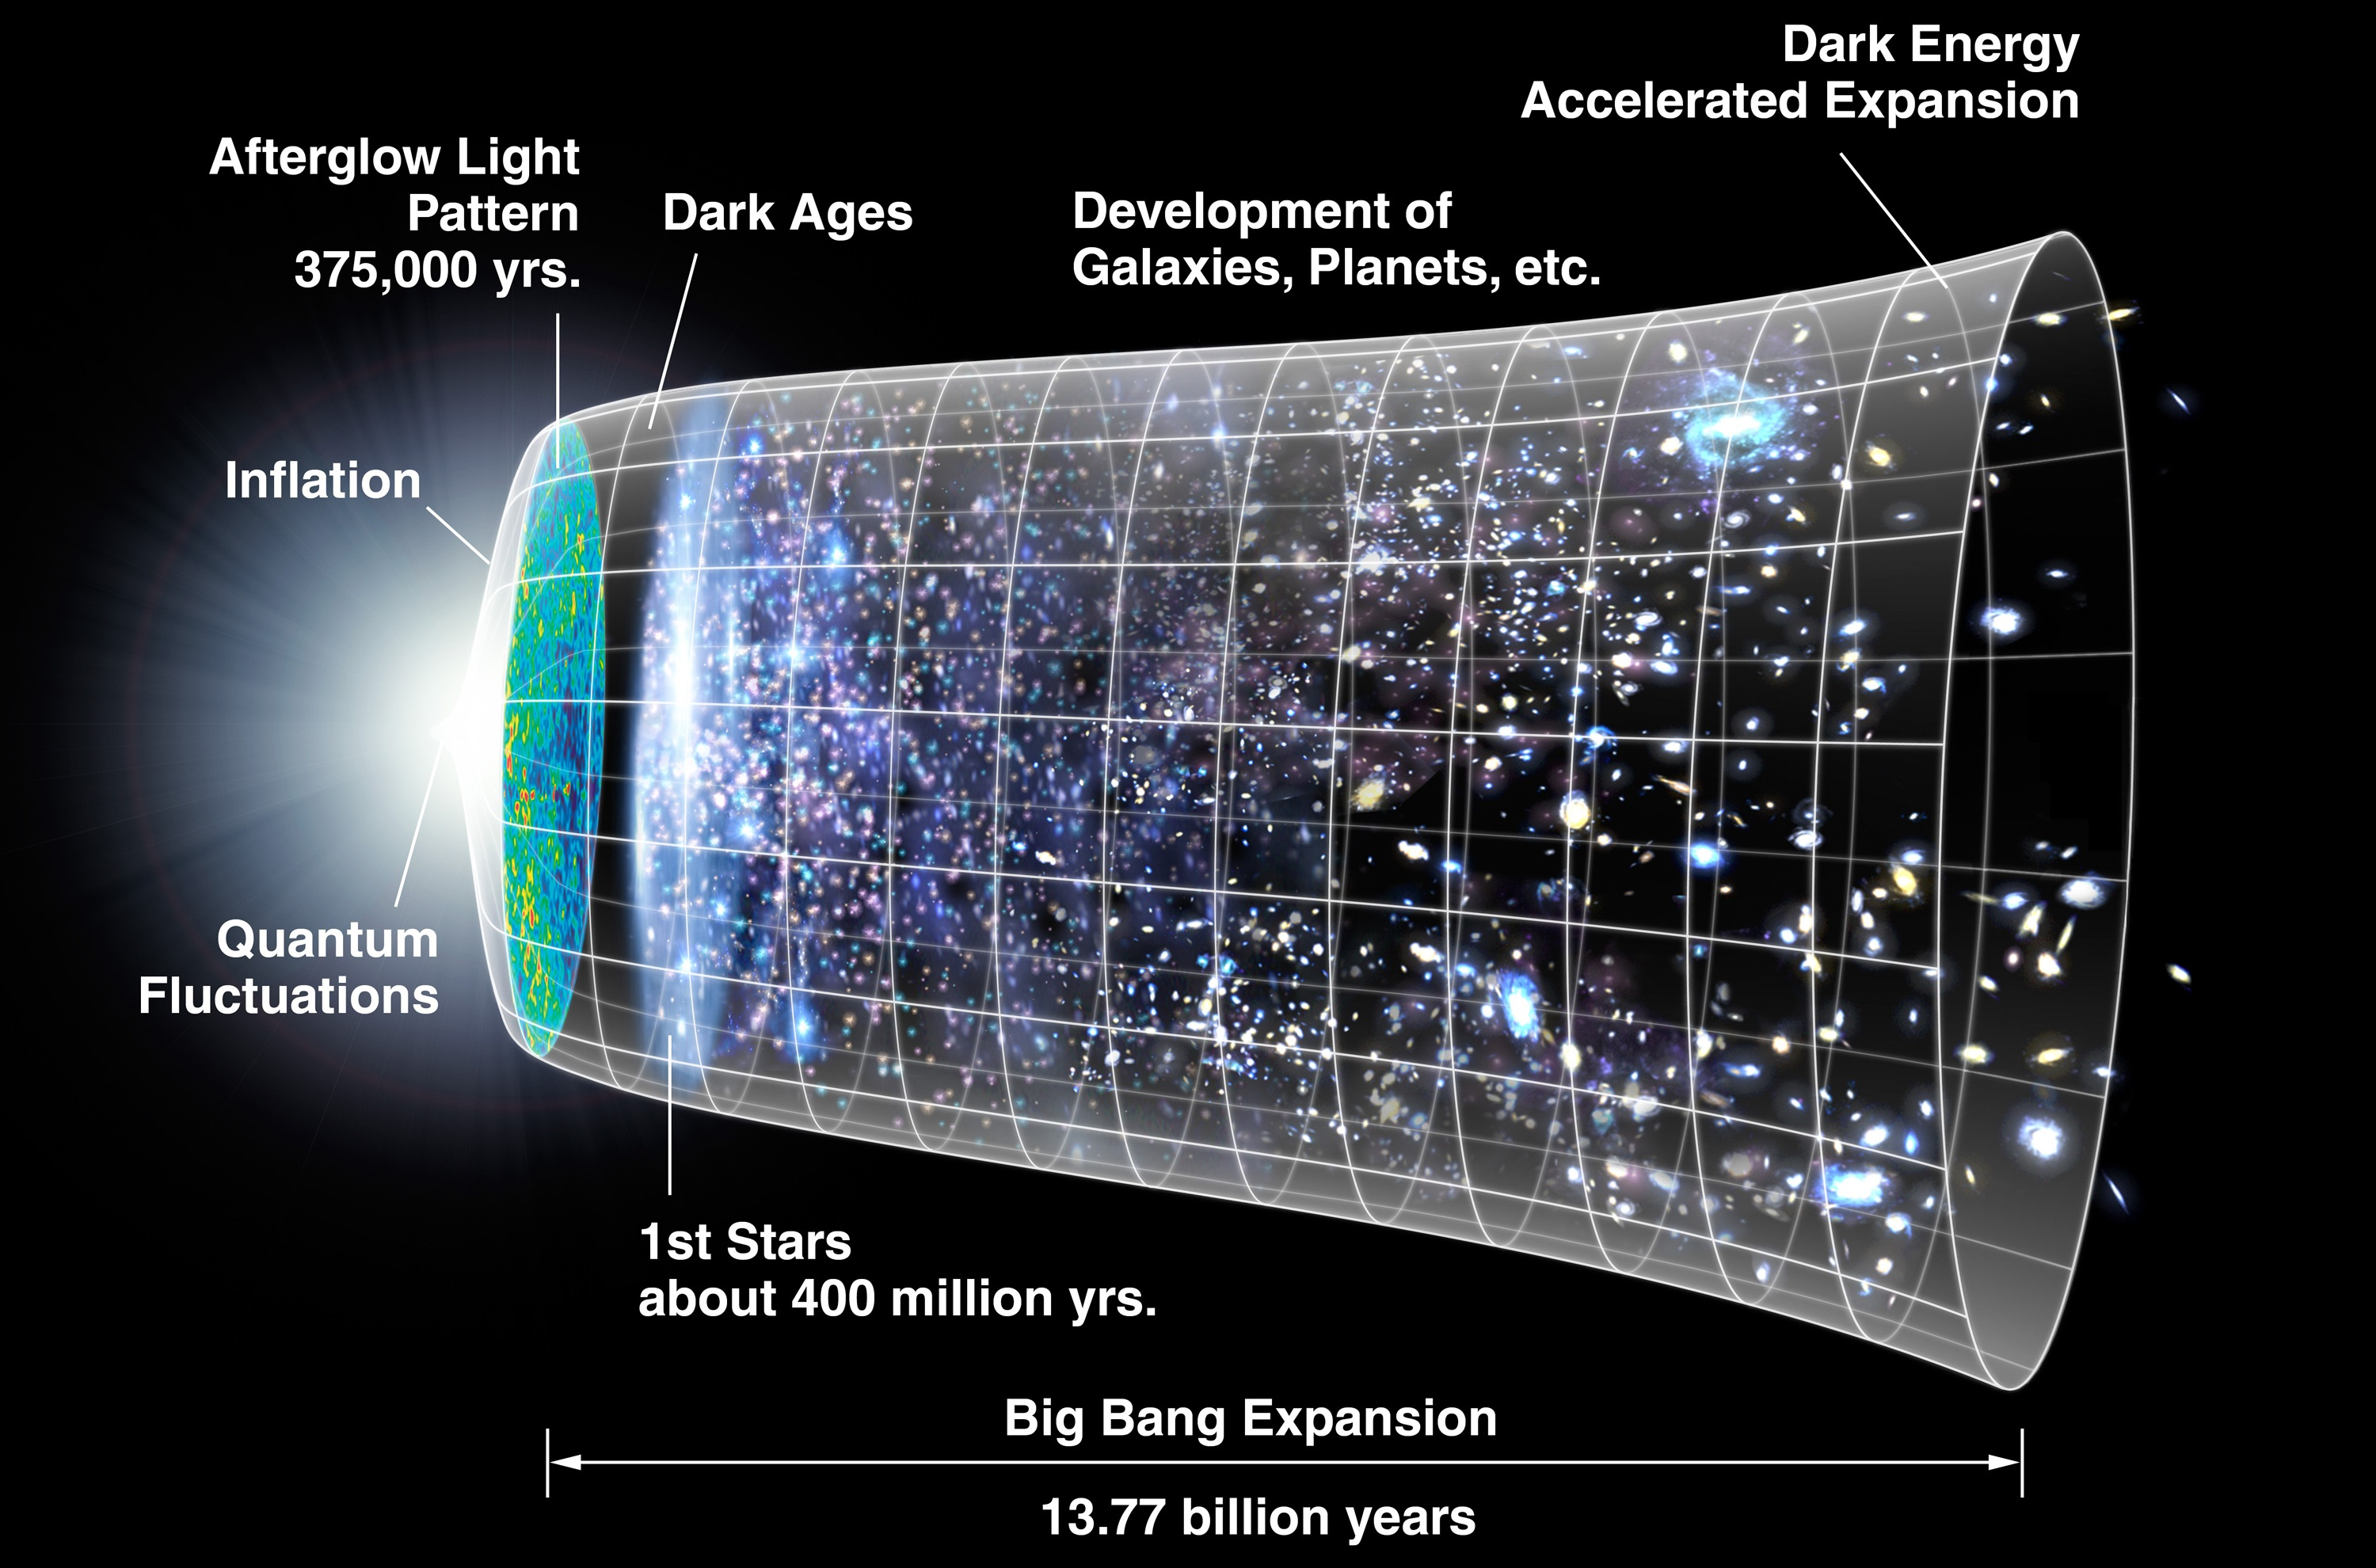
\includegraphics[width=\textwidth, angle=0]{Img/timescale.jpg}
\caption{Timeline of the universe. A representation of the evolution of the universe over 13.77 billion years. The far left depicts the earliest moment we can now probe, the far right represents the present time. Image Credits: NASA/WMAP Science Team}
\label{fig:timescale}
\end{figure}


The first helium nuclei has been synthesized from deuterium. At the same time, helium also can be synthesized, at higher temperatures, directly from four protons \citep{2000JRASC..94..198M,2000PhR...333..433P}. However, these helium nuclei (synthesized from four protons) were instantly annihilated by the highly energetic gamma rays, making the deuterium detour as the dominant source of the helium nucleosynthesis \citep{1969PhDT........85G,1969FMSp...12..111G,1979A&A....80...71A}. Lithium (the third ele­ment in the periodic table) was formed from the collisions of several helium nuclei. In other words, our universe, three minutes after the Big Bang, was built up of three fundamental el­ements: hydrogen, helium, and trace amount of lithium, with an approximate fractions $75 \%$ hydrogen, $75 \%$ helium, and merely $0.000000002 \%$ lithium \citep{1990BAAS...22.1214D, 2000INGN....3...14R,2000eaa..bookE4801.}. Afterwards, the universe cooled down enough to allow electrons (belongs to the lepton family) and protons to bound and form the first neutral atoms (hydrogen), this is known as the recombination epoch (100,000 years after the Big Bang) \citep{1991STIN...9211944D,1994PhDT.......131T,1996A&A...305..371P,2000fist.conf..229G}. About 150 million to 1 billion later, the temperature of the universe had dropped to $-270$ \textdegree{}C allowing the earliest structures (known as population III stars) to form \citep{1981ApJ...248..606B,1982ASIC...90..293O,1983Natur.304..514B,1983tasa.conf..108A,1984ASIC..117..253S,2000A&A...356..873A}. Figure \ref{fig:timescale} demonstrates the evolution, of the observable part, of our universe from the Big Bang to the present.



The previous two paragraphs try to summary the first phase of the element synthesis. The temperature of our universe had been cooled down too far, and heavier elements couldn't been synthesized from nuclear fusion with hydrogen, helium, and lithium. Nevertheless, our universe was still lacking the elements required to support life (e.g., carbon, nitrogen, oxygen), as well as the remaining elements in the periodic table. These elements were eventually built up, inside stars over billions of years. Therefore, and for the convenience of the reader a brief introduction to stars formation, stellar structure, and stellar evolutions are needed.




\section{Stars Formation}\label{formation}
The interior of the main-sequence (MS) or giant stars is in hydrostatic equilibrium; the balanced forces are an inward gravitational force and an outward nuclear force, with a temperature of the order of ${10^7}$~K \citep{leblanc2010introduction}. The thermodynamic conditions, characterized by the variables temperature and pressure, are sufficient for nuclear fusion to occur, which in term lead to produce adequate energy preventing any further collapse of the star. Stars have very different structures, as they evolve in their lives; however, MS stars have a general structure that is roughly the same and can be illustrated by our sun (see Figure \ref{fig:sun}). Like all stars, our sun is mainly made up of hydrogen and helium, with main parts as follow \citep{1972RvGSP..10..395G}:



\begin{figure}[!ht]
\centering
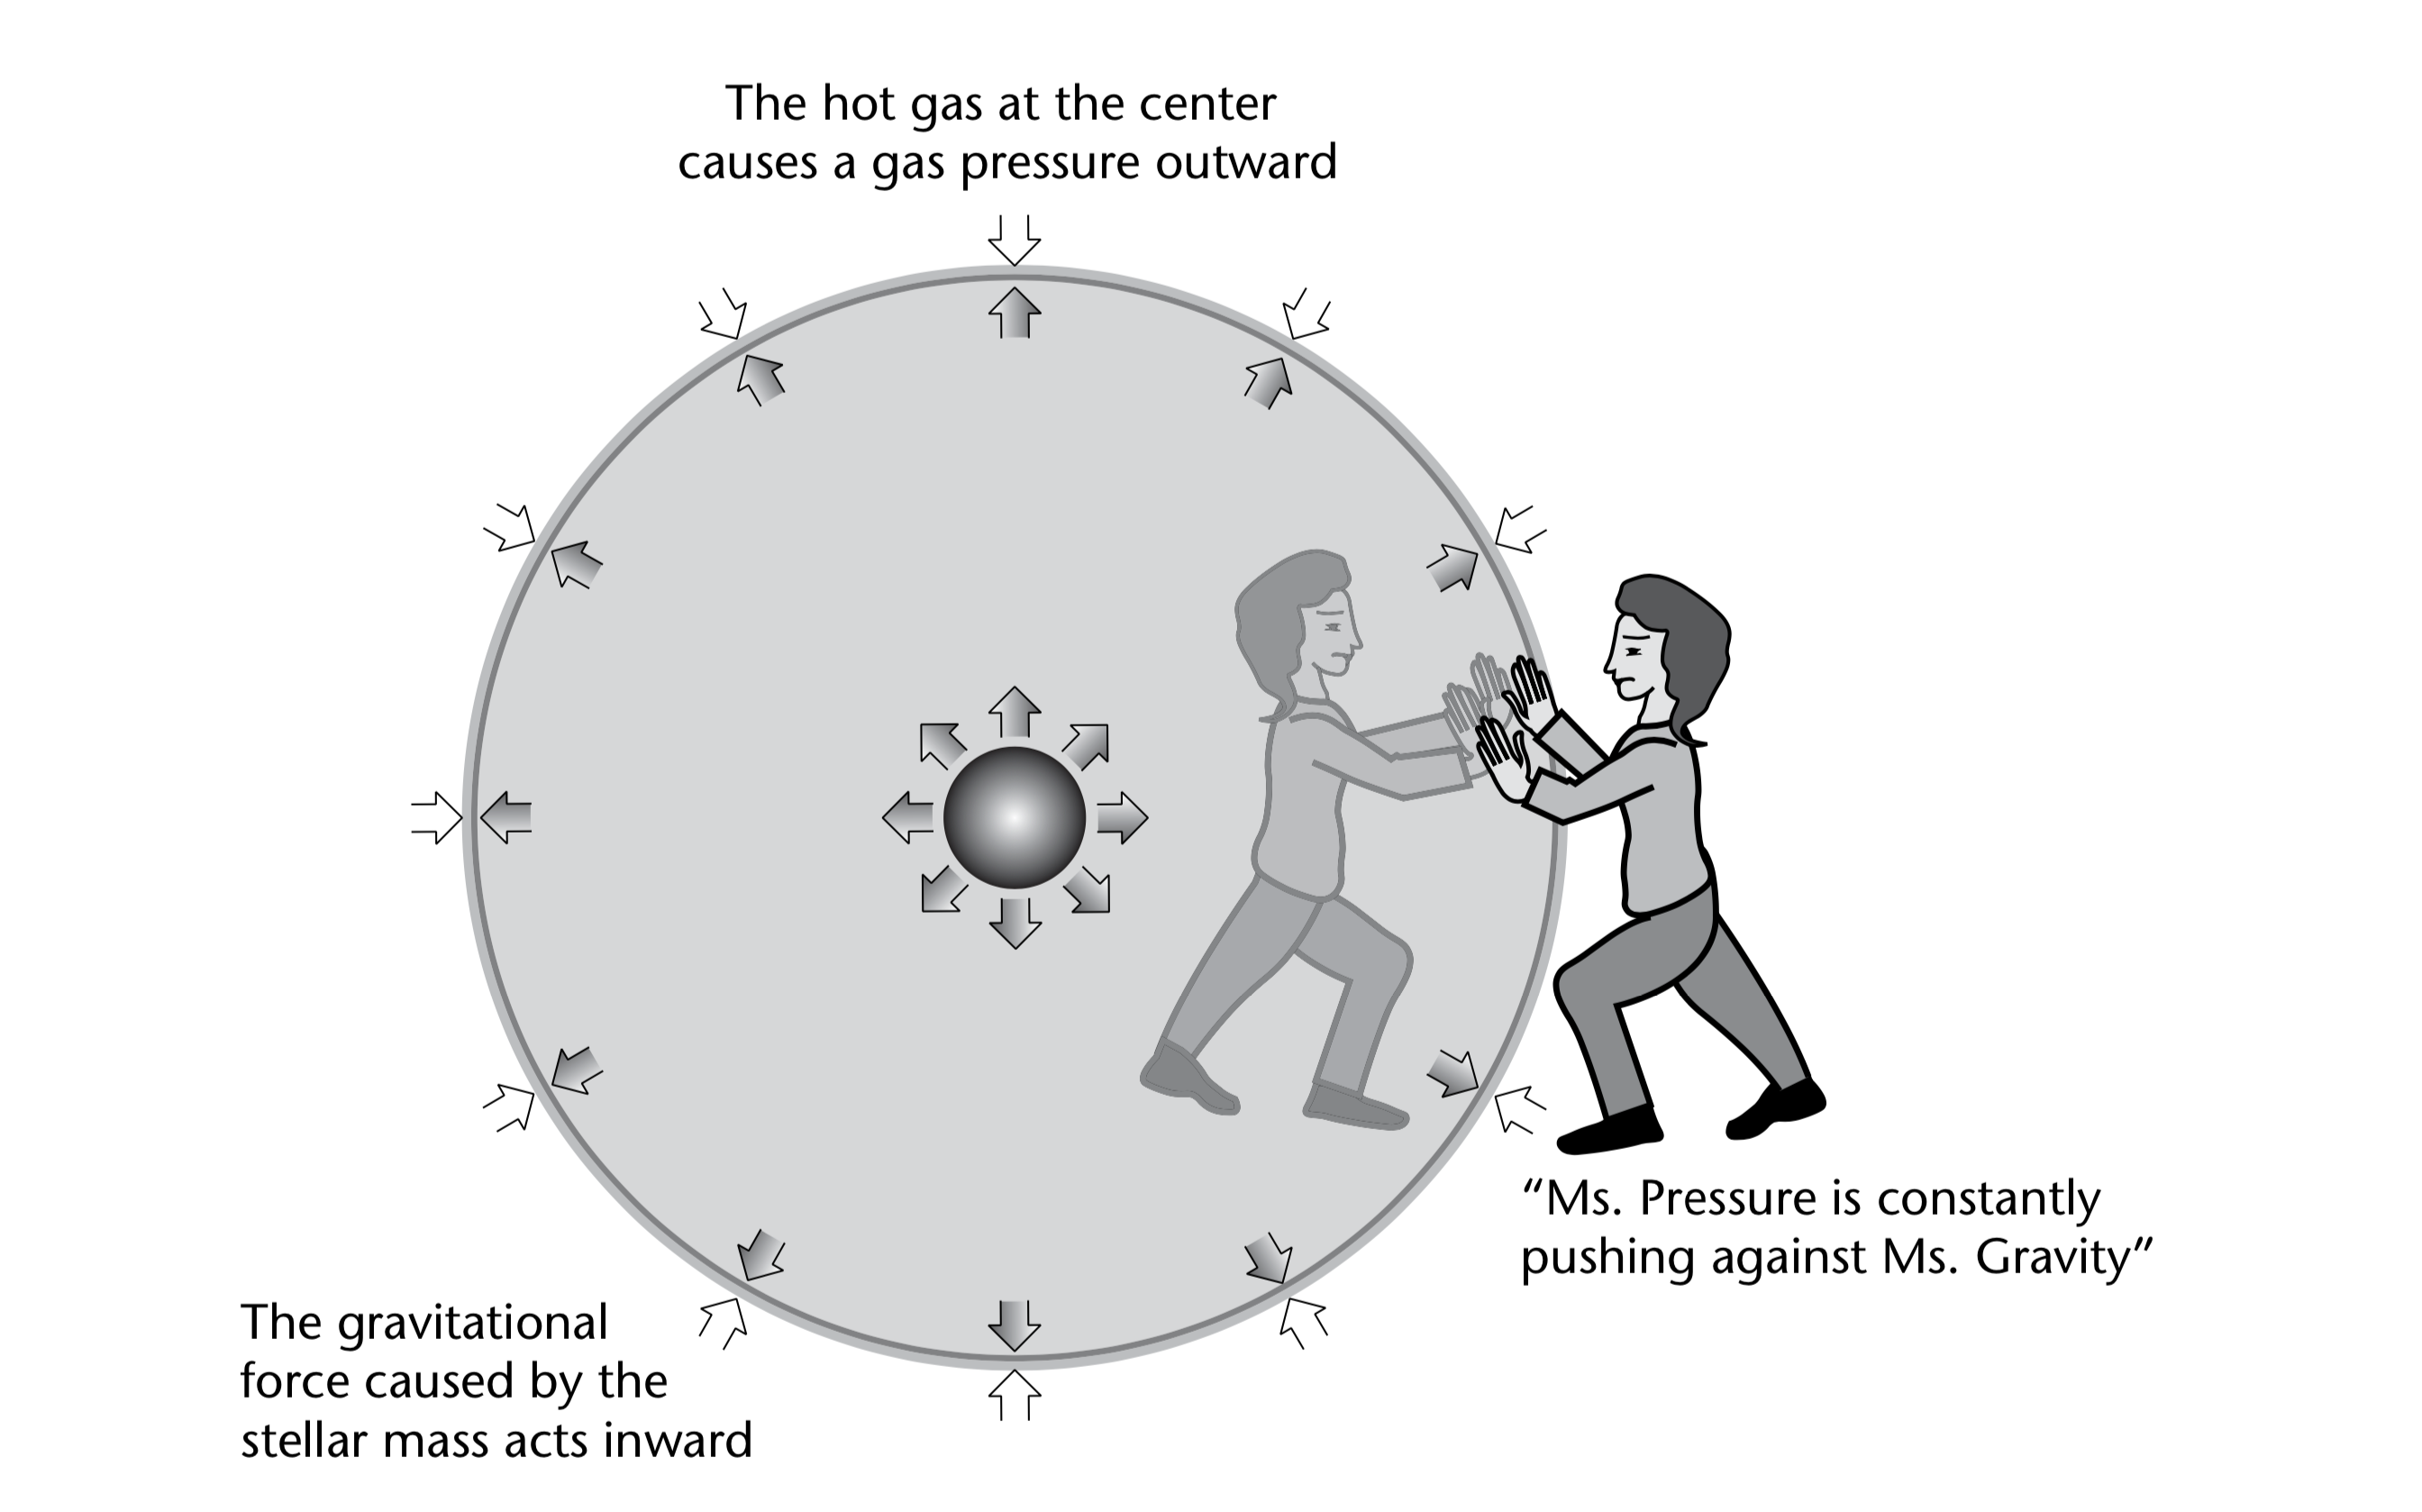
\includegraphics[width=\textwidth, angle=0]{Img/gravity_vs_nuclear.png}
\caption{A schematic view of the hydrostatic equilibrium. The outward force has to balance the inward force. Only then does a star remain in equilibrium and neither collapses nor flies apart. Credits: Peter Palm} 
\label{fig:sun}
\end{figure}


\begin{figure}[!ht]
\centering
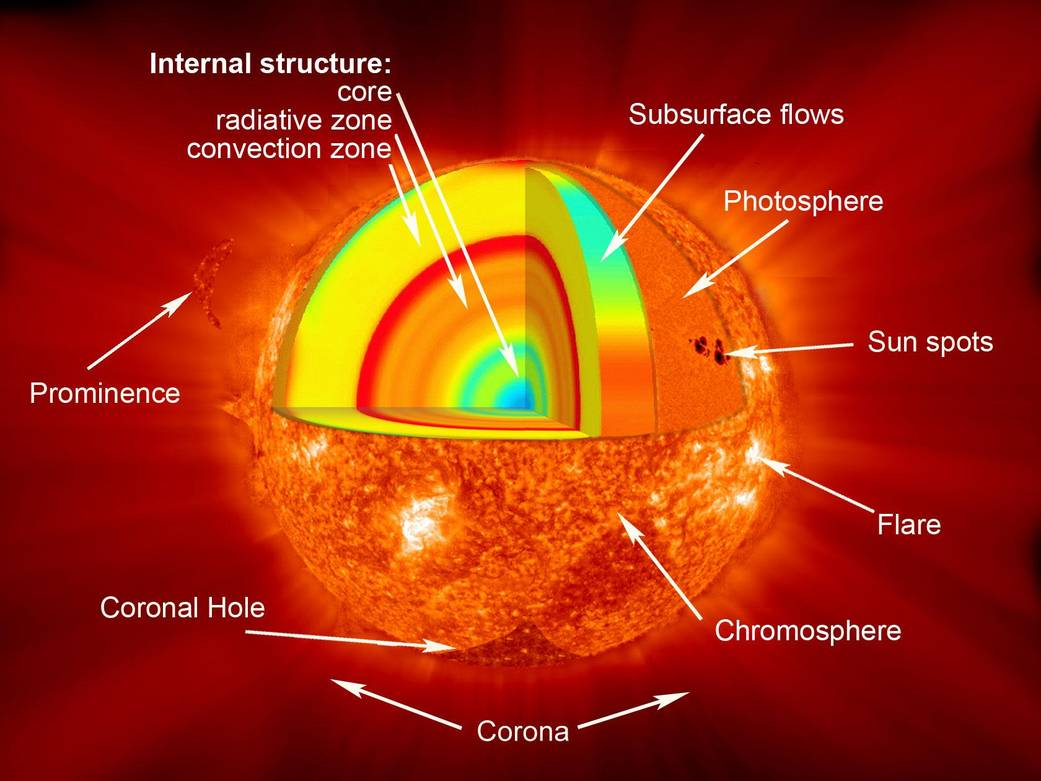
\includegraphics[width=\textwidth, angle=0]{Img/sun_layers.jpg}
\caption{A schematic view of the Sun's structure as an illustrative example of stellar structure. Credits: NASA/Goddard} 
\label{fig:sun}
\end{figure}



\begin{description}
\item[\textbf{Interior}]: This is the part of the star which is below its surface and cannot be directly seen \citep{2019RSPTA.37790152A}. Depending on the types of transport of energy, which is in action, the stellar interiors can be divided into:
\begin{enumerate}
\item \textbf{The Core}: This is the region located inside the star where temperature and pressure are sufficient to ignite nuclear fusion. The process of converting hydrogen into helium and the release of a tremendous amount of energy occurs in the core. More massive stars will have larger, hotter cores \citep[e.g.,][]{1970AcA....20..195P,2019JPhG...46f5201V}.
\item\textbf{The Radiative Zone}: This is the region where energy transportation is dominated by electromagnetic radiation (gamma rays). The radiative zone extends from a depth of 515,000 km to 200,000 km, concerning the surface of the Sun \citep[e.g.,][]{2006ApJ...650.1208M}.
\item \textbf{ The Convection Zone}: Here the energy transport mechanism is convection. This zone is the outermost layer of the interior, and it extends from  200,000 km up to the visible surface \citep[e.g.,][]{2018csc..confE..46H, 2018PhPl...25i0702Y}.
\end{enumerate}

\item[\textbf{Photosphere}]: Looking to the Sun, the view becomes more and more opaque, just like seas. The point where the Sun appears to become completely opaque is called the photosphere. Thus, the photosphere may be thought of as the imaginary surface from which the solar light that we see appears to be emitted \citep[e.g.,][]{2018A&A...620A.183J,2019ApJ...874..103K}.

\item [\textbf{Atmosphere}]: This is the outer part of the sun, where the gamma rays finally reach the space.
\end{description}



\section{Stellar Evolutions}\label{evolution}
Fusion is the dominant type of nuclear reactions occurring in stars. Inside the cores of these stars, a variety of different nuclear fusion reactions occur, upon their mass and composition. The resulting atomic nuclei, in term of mass, are lighter than the sum of the reactant elements. This mass difference is released as electromagnetic energy according to the well known Einstein's relation for the equivalence between energy and mass (E = Mc$^{2}$). Based on the dominate fusion nuclear reactions, stars have different stellar evolutionary phases. Here, we try to give brief introduction to these phases.



\subsection{H-Burning Phase}
The H-burning mechanism is primarily the nuclear fusion of four hydrogen nuclei ($^{1}$H) into one helium nucleus ($^{4}$He). The amount of this fuel (hydrogen) is consumed at a lower rate than in any other evolutionary phase; therefore, the H-burning lifetime, for all stars, is longer than the other evolutionary phases (e.g., the H-burning phase is longer by a factor of 100 than the He-burning stage) \citep[e.g.,][]{2010JKPS...56.1673C}. The fusion of these four H nuclei can be achieved through two possible reaction chains \citep[namely the p-p chain and the CNO cycle,][]{2018Natur.562..505B, 2018PhP....20..124W}. These two reaction chains usually occur simultaneously, but with relative efficiencies, depending on the stellar mass and the temperature of its core \citep[e.g.,][]{1990ApJS...74..463C}.


\subsubsection{The p-p Chain}
The first reaction in the p-p chain (pp I) requires that protons experience a $\beta^{+}$ decay; since it is impossible to form a bound system with two protons. This reaction can occur only if the protons are brought together by a nuclear collision (see Figure \ref{ppchain}). During this short timescale collision, one of these collided protons has the chance to $\beta^{+}$ decay, and then convert into a neutron, a positron, and a neutrino. The neutron can then be captured by the other proton to form a deuteron. This process is governed by weak interaction and therefore has a low probability of occurring; its cross-section is in fact quite low ($\approx 10^{-23}$ barn; 1 barn = $10^{-24}$ cm$^{2}$). The pp I chain therefore begins to be important only when the core temperature is of the order of 5 $\times 10^{6}$ K \citep{2018Natur.562..505B}. Until a temperature of the order 8 $\times 10^{6}$ K is reached, the reactions producing $^{3}$He are more frequent than those consuming $^{3}$He and as a consequence the abundance of $^{3}$He increases. When this temperature is achieved, the nuclear reactions $^{3}$He + $^{3}$He and $^{3}$He + $^{4}$He become effective, so decreasing the $^{3}$He abundance. The relative frequency of pp II and pp III depends strongly on the temperature. In particular, the $^{3}$He + $^{4}$He reaction becomes competitive with respect to $^{3}$He + $^{3}$He for T $\approx 15 \times 10^{6}$K \citep{leblanc2010introduction}. As a general rule, with increasing temperature the importance of the pp II and pp III increases with respect to pp I if there is a sufficient concentration of the $^{4}$He (either produced by the pp I or primordial). In addition, pp III gradually becomes more important than pp II.







\textbf{pp I}

$^{1}$H + $^{1}$H $\longrightarrow$ $^{2}$D + $e^{+}$ +
$\nu_{e}$


$^{2}$D + $^{1}$H $\longrightarrow$ $^{3}$He + $\gamma$

$^{3}$He + $^{3}$He $\longrightarrow$ $^{4}$He + $^{1}$H +
$^{1}$H

\textbf{pp II}

$^{3}$He + $^{4}$He $\longrightarrow$ $^{7}$Be + $\gamma$


$^{7}$Be + $e^{-}$ $\longrightarrow$ $^{7}$Li + $\nu_{e}$


$^{7}$Li + $^{1}$H $\longrightarrow$ $^{4}$He + $^{4}$He

\textbf{pp III}

$^{3}$He + $^{4}$He $\longrightarrow$ $^{7}$Be + $\gamma$

$^{7}$Be + $^{1}$H $\longrightarrow$ $^{8}$B + $\gamma$

$^{8}$B $\longrightarrow$ $^{8}$Be + $e^{+}$ + $\nu_{e}$


$^{8}$Be $\longrightarrow$ $^{4}$He + $^{4}$He


\begin{figure}[!ht]
\centering
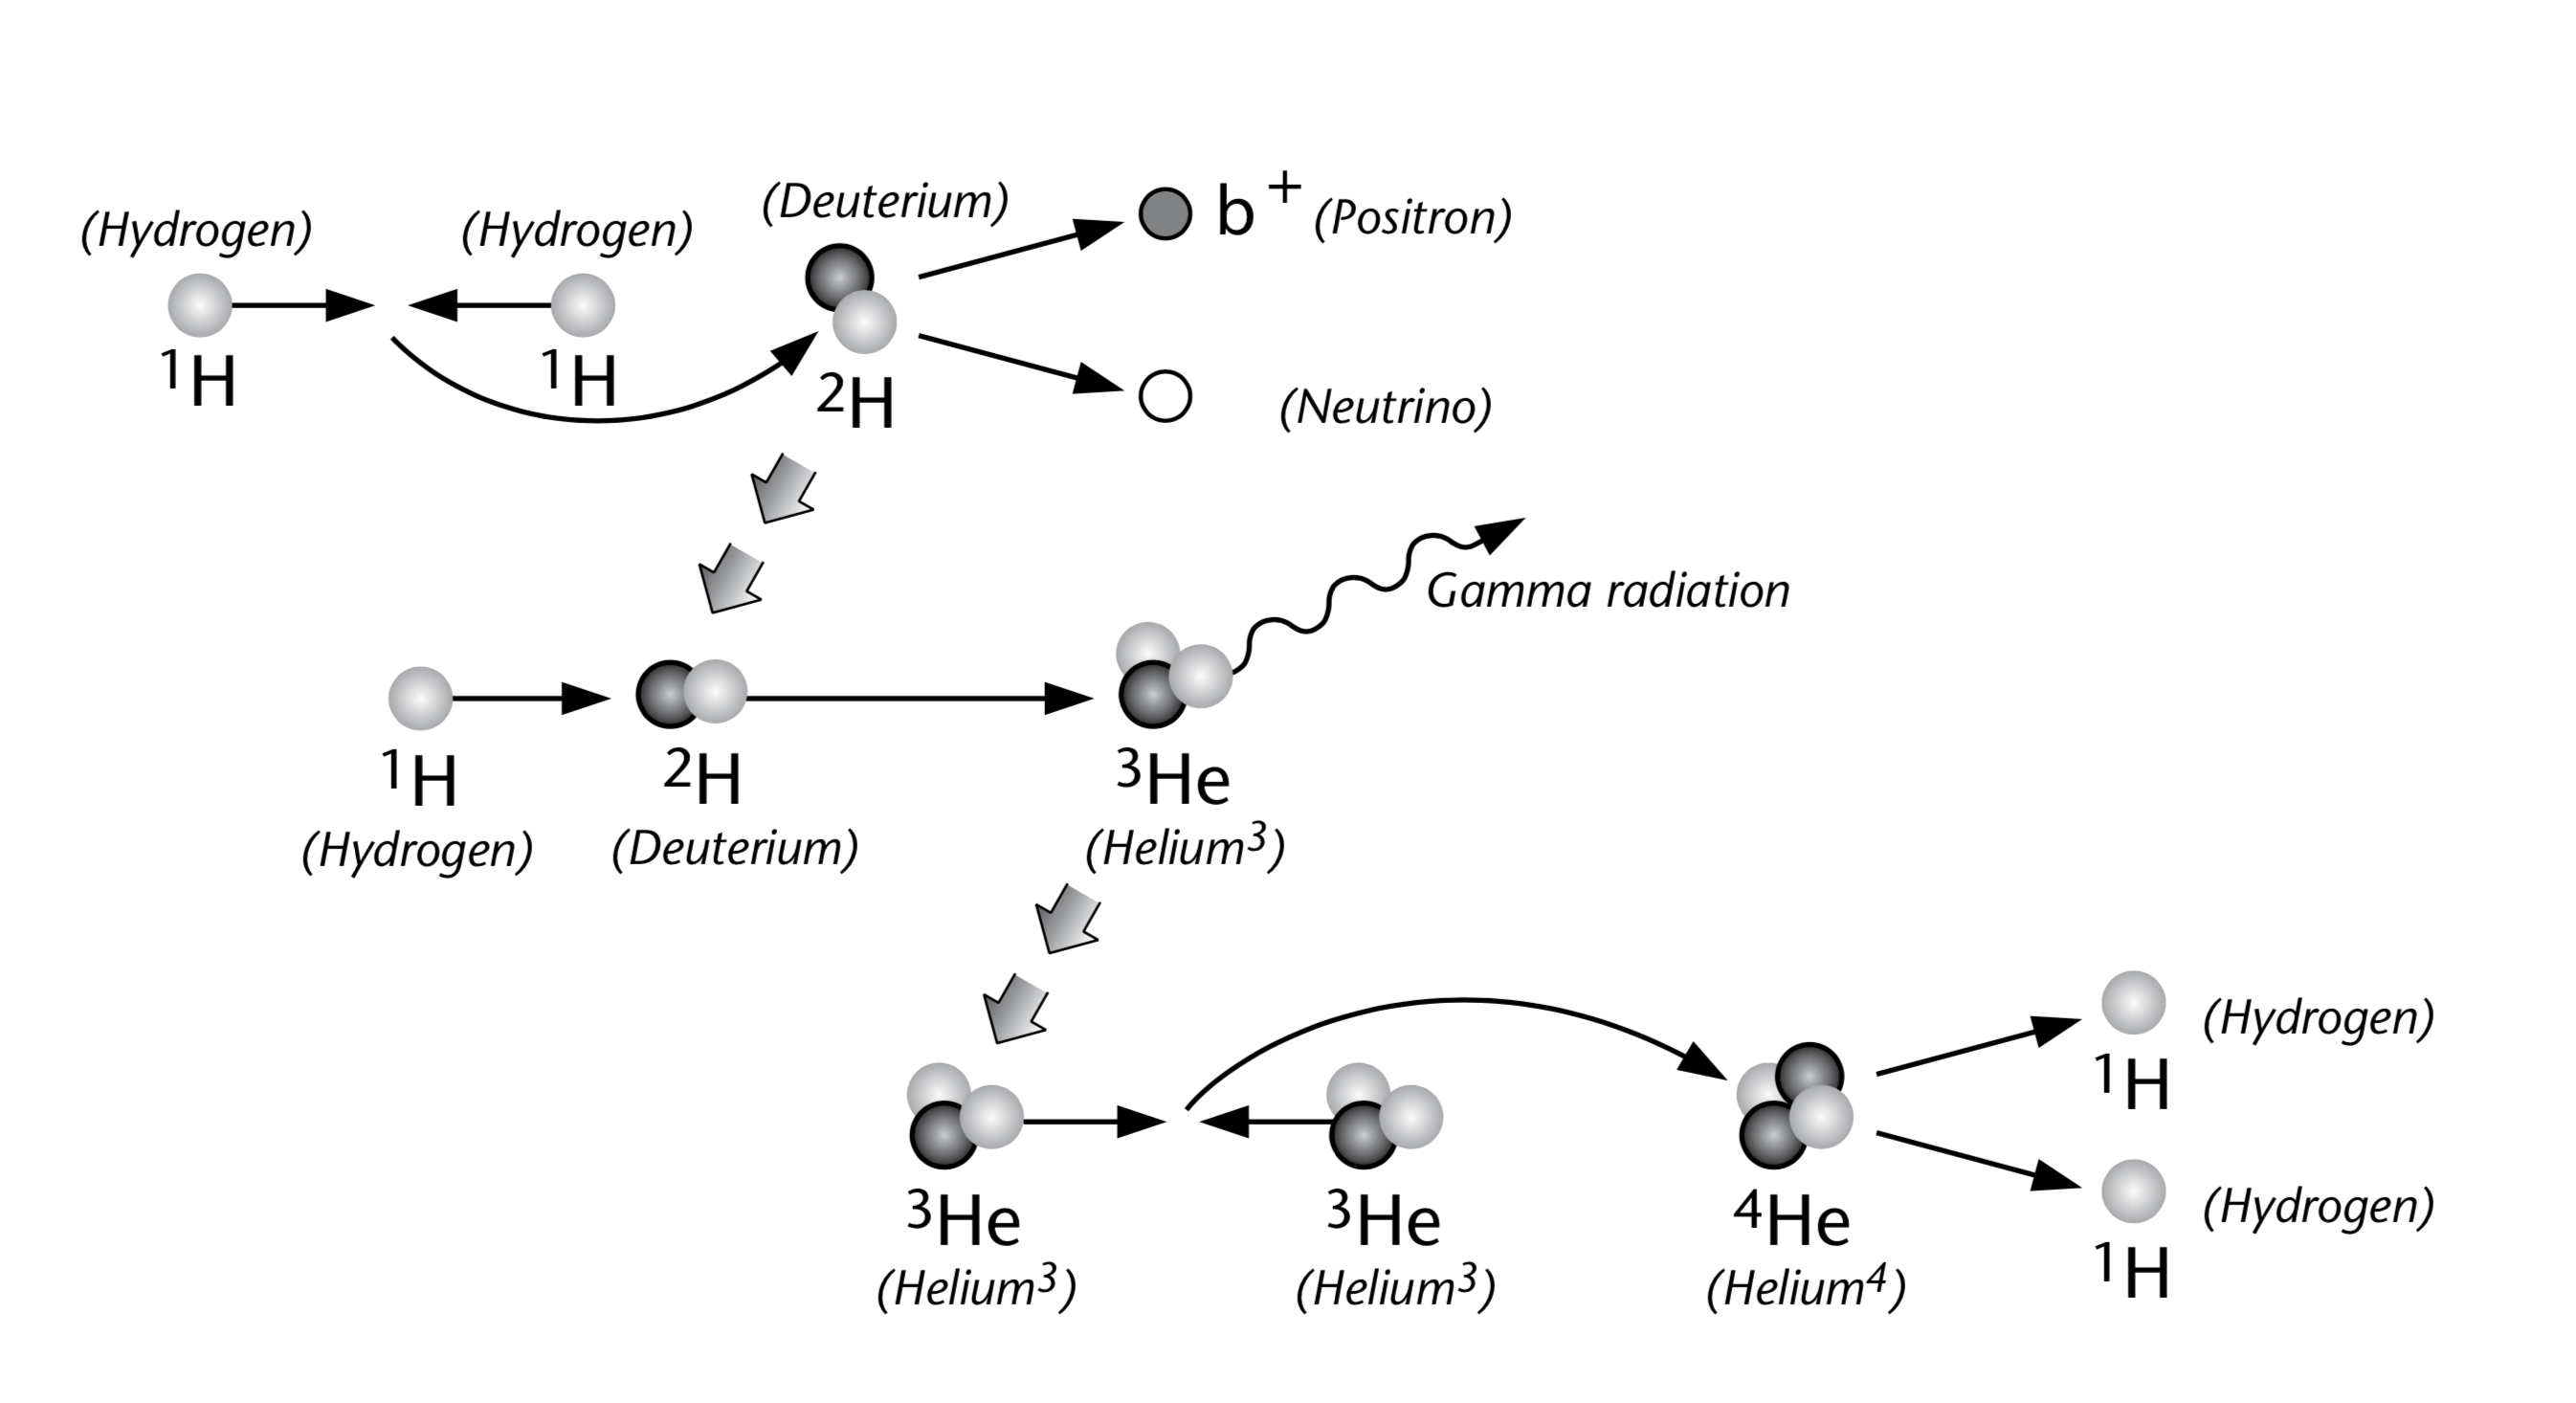
\includegraphics[width=\textwidth, angle=0]{Img/ppchain.png}
\caption{Schematic view of the proton-proton chain, fusion of four hydrogen nuclei into one helium nucleus. This fusion happened in three steps, energy is released in every step. Credits: Peter Palm} 
\label{ppchain}
\end{figure}



\subsubsection{The CNO Cycle}
The CNO cycle is a combination of two separate cycles; CN cycle and NO cycle (see Figure \ref{cno}). The existence of some isotopes (e.g., $^{12}$C, $^{15}$N, $^{16}$O) are crucial for either cycles to take place \citep[see below the reaction networks involved in this process,][]{2018PhP....20..124W}. Carbon and nitrogen are subject to be produced and destroyed throughout these cycles; these elements play the role ofcatalysts. In the CN cycle, the isotopes of C and N act as catalysts, and so behave as "secondary elements". As a consequence the cycle can start almost from any reaction if the involved isotope is present, and during a complete loop around the cycle the isotope is consumed and then produced again.

\vspace{2mm}
\textbf{CN cycle}

$^{12}$C + $^{1}$H $\longrightarrow$ $^{13}$N + $\gamma$

$^{13}$N  $\longrightarrow$ $^{13}$C + $e^{+}$ + $\nu_{e}$

$^{13}$C + $^{1}$H $\longrightarrow$ $^{14}$N + $\gamma$

$^{14}$N + $^{1}$H $\longrightarrow$ $^{15}$O + $\gamma$

$^{15}$O $\longrightarrow$ $^{15}$N+ $e^{+}$ + $\nu_{e}$

$^{15}$N+ $^{1}$H $\longrightarrow$ $^{12}$C + $^{4}$He


\begin{figure}[!ht]
\centering
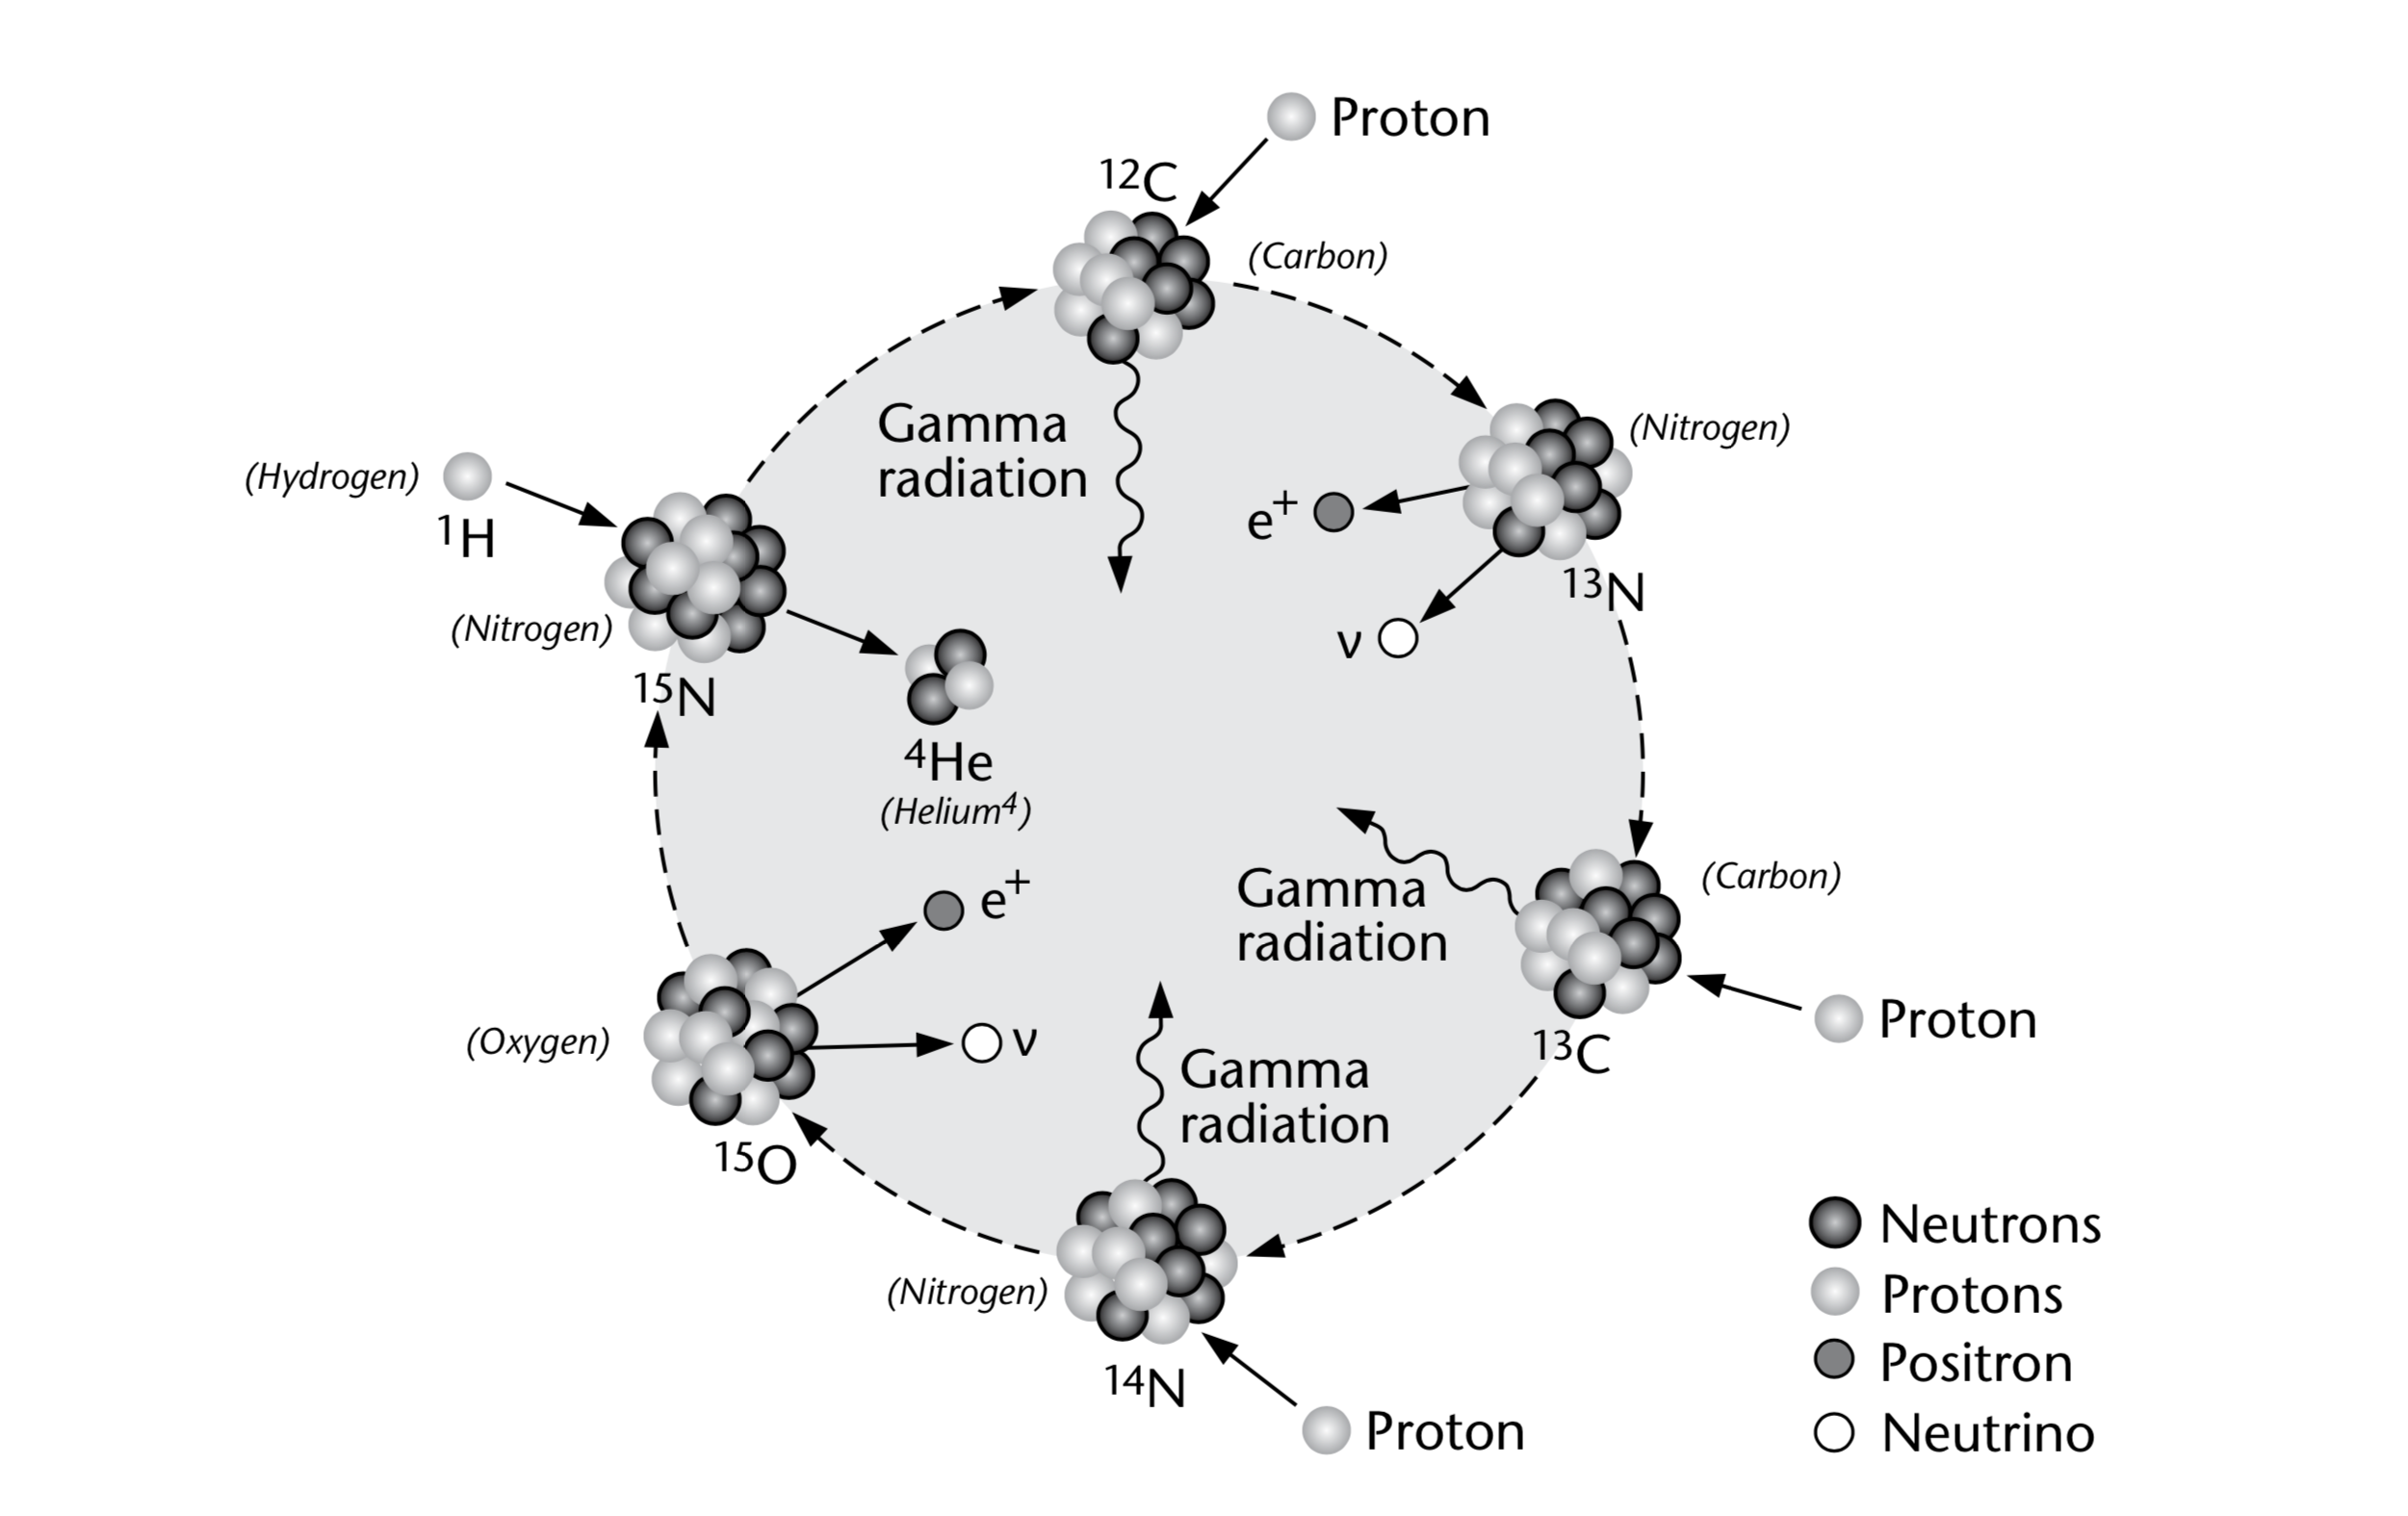
\includegraphics[width=\textwidth, angle=0]{Img/CNO.png}
\caption{Schematic view of the CNO cycle. Helium is produced in six steps, energy is released in every step. Credits: Peter Palm} 
\label{cno}
\end{figure}


\textbf{NO cycle}

$^{15}$N+ $^{1}$H $\longrightarrow$ $^{16}$O + $\gamma$

$^{16}$O + $^{1}$H $\longrightarrow$ $^{17}$F + $\gamma$

$^{17}$F  $\longrightarrow$ $^{17}$O + $e^{+}$ + $\nu_{e}$

$^{17}$O + $^{1}$H $\longrightarrow$ $^{14}$N + $^{4}$He


\vspace{2mm}
However, this does not mean that the concentrations of the different isotopes will be unchanged as the final abundances depend strongly on the relative rates of the nuclear reactions in the cycle. Only at a high enough temperature (T$\approx 15\times10^{6}$K) the isotopes achieve their equilibrium abundance; the rate of the production is exactly equal to the rate of the destruction. At this point, the abundance of each isotope is inversely proportional to the nuclear cross-section of its destruction. Hence the slowest reaction of the CNO cycle is $^{14}$N (p,$\gamma) ^{15}$O, because it has the largest cross-section. \footnote{Here we have introduced the compact notation $^{14}$N (p,$\gamma) ^{15}$O instead of $^{14}$N + $^{1}$H $\longrightarrow$ $^{15}$O + $\gamma$}. The most abundant element in the CNO cycle processed material is $^{14}$N \citep{2016NatSR...622038S}. The branching ratio of the proton captures by $^{15}$N, producing respectively $^{16}$O and $^{12}$C, is of the order of $10^{-4}$ \citep{2018PhP....20..124W}, thus the amount of $^{16}$O produced by proton capture on $^{15}$N is negligible. Nevertheless, the small production of $^{16}$O through this channel is important because it allows the $^{16}$O nuclei originally present to take part in the cycle as well, as they are transformed into nitrogen via the NO cycle \citep{2016NatSR...622038S, 2018PhP....20..124W}. The temperature sensitivity of the complete CNO cycle is much larger than that of the p-p chain, where $\epsilon_{CNO} \propto $T$^{18}$ at T$\approx 10 \times 10^{6}$K. This means that the p-p chain dominates at low temperatures (T$\leq 15 \times 10^{6}$K) in stars with mass lower than $\approx 1.3 M_{\odot}$, while the CNO cycle dominates at higher temperatures for larger stellar masses. In Figure \ref{temperature}, the trends of both $\epsilon_{pp}$ and $\epsilon_{CNO}$ with temperature are shown. At the center of the sun $\epsilon_{pp} \backslash \epsilon_{CNO} \approx
10$, so that the contribution of the CNO cycle to the whole energy budget is of the order of 10 per cent \citep{2011A&A...533A..66C,2016NatSR...622038S,2018PhP....20..124W}.


\begin{figure}[!ht]
\centering
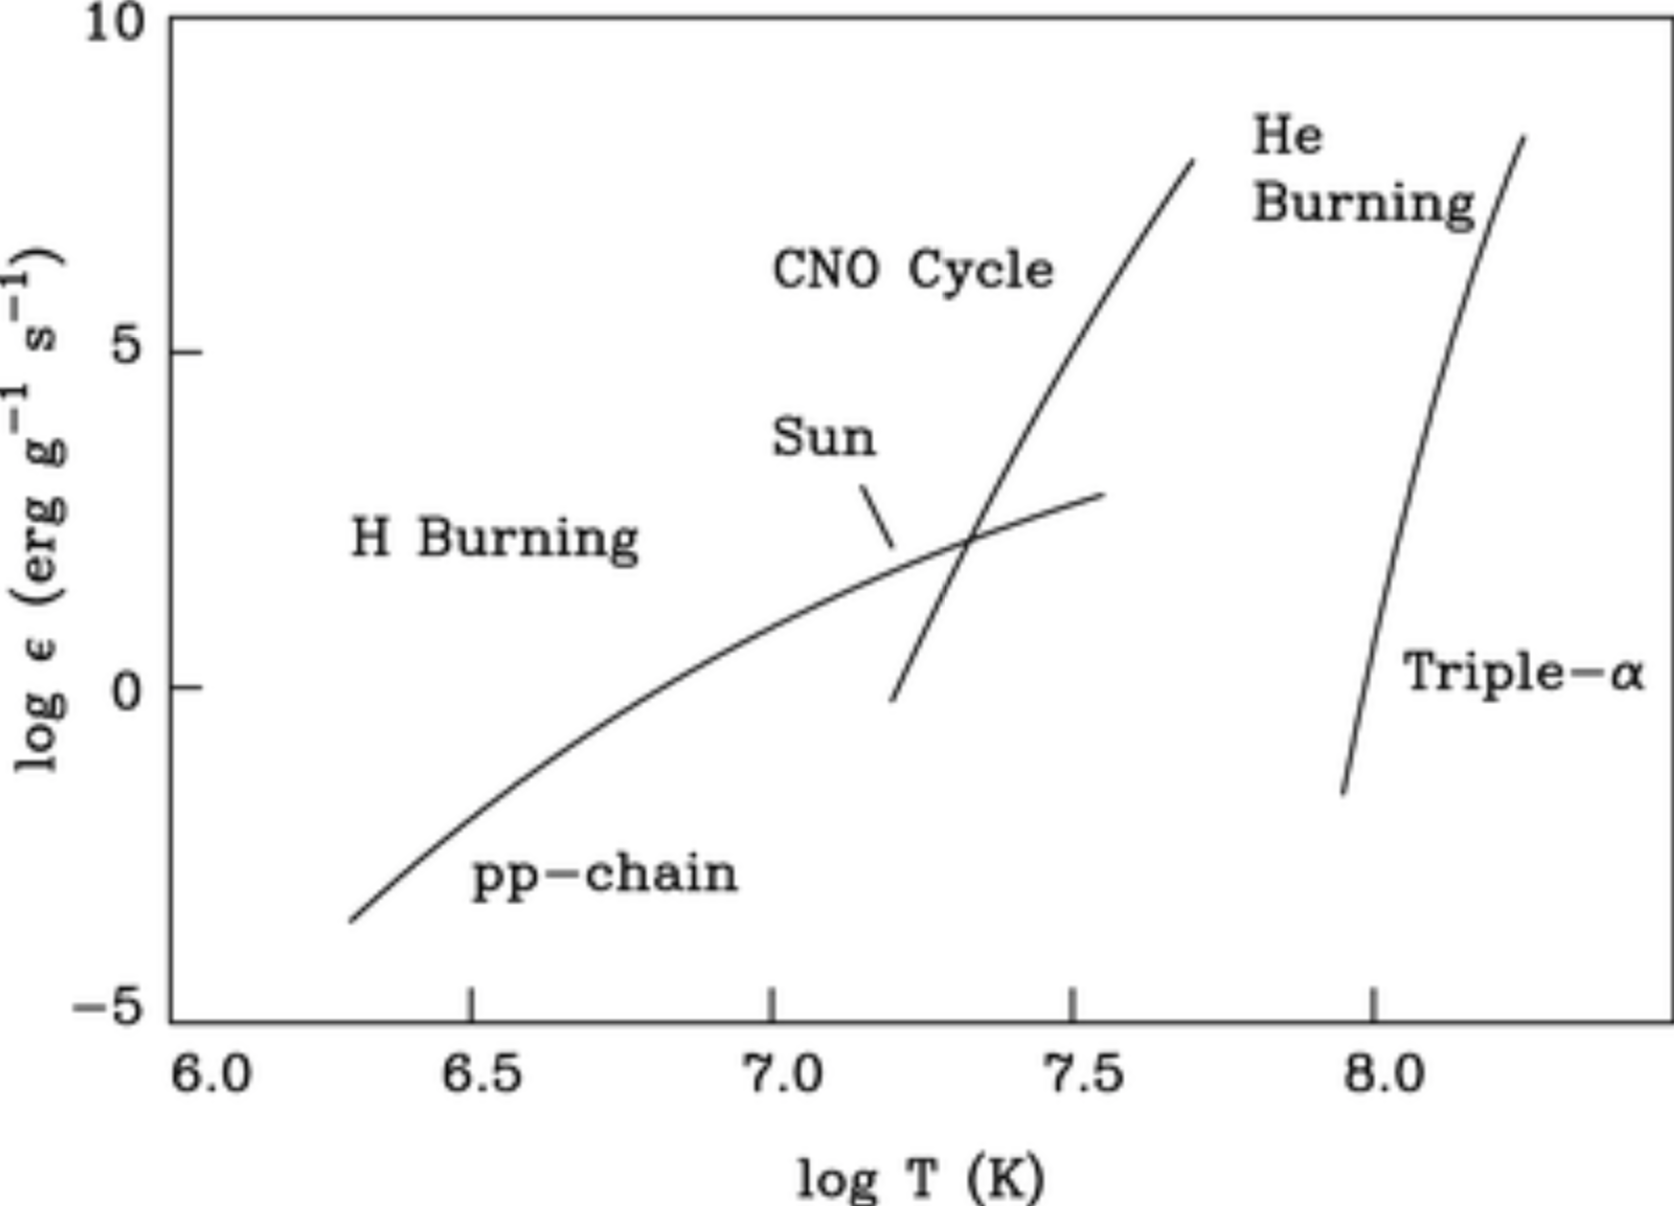
\includegraphics[width=\textwidth, angle=0]{Img/pp.png}
\caption{The nuclear energy generation in units of erg $g^{-1}~s^{-1}$ as a function of the temperature for the p-p chain and the CNO cycle. The open circle marks the location of the sun in this diagram. Credits: LEBLANC/An introduction to stellar astrophysics} 
\label{temperature}
\end{figure}




\subsection{The Helium Burning Phase}

The helium burning phase is the second stage of a stellar evolution. Unlike during the H-burning phase (discussed previously), the nuclear-physical processes at work in stars of different masses, during the main core He-burning stage are quite similar. The first and fundamental reaction in the He-burning process is the production of $^{12}$C from the fusion of three $^{4}$He nuclei. This reaction is called the triple alpha ($3\alpha$) reaction (see Figure \ref{temperature}). A triple collision being of very low probability, this reaction usually occurs in two separate steps \citep{1955ApJS....2....1H,1960AJ.....65T.490H,1970ApJ...161..587I,2019ApJ...878...49W}.

\vspace{2mm}
$^{4}$He + $^{4}$He $\longrightarrow$ $^{8}$Be (-93.7 keV)

$^{8}$Be + $^{4}$He $\longrightarrow$ $^{12}$C + $\gamma$ (+7.367 MeV)
\vspace{2mm}

The first reaction is endothermic or endoergic, meaning that in a short time, ($\sim$ $10^{-16}$s) $^{8}$Be decays back into two $\alpha$ particles. The possibility of the second reaction is therefore extremely low. However, when the interior temperature rises (of the order of $\sim 1.2\times10^{8}$K) the probability of the second reaction increases \citep{2010ApJ...718..357T,2011PhLB..695..324D,2017APh....87...40A,2019APh...105...13H}. The other nuclear reactions involved in the He-burning process are:

\vspace{2mm}
$^{12}$C $+ \alpha \longrightarrow$ $^{16}$O + $\gamma$

$^{16}$O + $\alpha$ $\longrightarrow$ $^{20}$Ne + $\gamma$

$^{20}$Ne + $\alpha$ $\longrightarrow$ $^{24}$Mg + $\gamma$

$^{24}$Mg + $\alpha$ $\longrightarrow$ $^{28}$Si + $\gamma$
\vspace{2mm}

Only the first two reactions, together with the $3\alpha$ reaction, are really important, a relevant consequence of the He-burning process is to transform He into a mixture of $^{12}$C and $^{16}$O with traces of $^{20}$Ne. Unfortunately, the alpha capture by $^{12}$C has a resonance and a very low cross-section ($\sim 10^{-17}$ barn) at low energies. Consequently the nuclear parameters are difficult to measure experimentally or to calculate by theoretical analysis.


\subsection{The Advance Evolutionary Phase}
The giant onion is the next evolutionary phase ; after the exhaustion of Helium in the core. This phase is well clear in the asymptotic giant branch (AGB) stars \footnote{corresponds to the He-shell burning phase. The designation asymptotic comes from the fact that in low-mass AGB stars, the effective temperature-luminosity relationship is very similar, a little bit slightly hotter, to that of low-mass stars, the so-called red giant branch stars (RGB) stars. For more massive stars the term asymptotic has no morphological significance}. After He-exhaustion, He-burning shifts to shell around the CO core, whose mass size increases as consequence of the convection of helium to carbon and oxygen in the He-burning shell \citep{1962AJ.....67Q.577H, 1962ApJ...136..166H, 1968PThPh..39.1432S,1976ApJ...207..209L,1970PThPh..44..599S,1997ApJ...489..772I,2006A&A...448..717S}. The overlying H-burning shell, which has burnt outwards for some time, extinguishes due to the expansion and consequence drop of its temperature. The latter drop is caused by the onset of He-burning in the shell. In low-mass stars, the onset of the He-burning induces a temporary drop of the surface luminosity and the star crosses the same region of the H-R diagram three times (as during the RGB bump phase). As a consequence, there is a good probability of observing an AGB star during this phase, which is called the AGB clump. This is indeed the case in well-populated old galactic stellar system \citep{1991ApJS...76..911C,2001MmSAI..72..703D}. In these stars, the large energy flux produced by the He-burning shell causes the base of the H-rich shell to expand and cool, so that H-burning in the shell immediately is switched off. When this occurs, the outer convection zone penetrates inward, into the H-depleted zone. This process is known as the second dredge up \citep{1979ApJ...232..831B}. For lower mass objects, H-burning remains quite efficient, and prevents the outer convection from penetrating deeper into the star \citep[therefore the second dredge up dose not occur,][]{1979ApJ...232..831B}.



\begin{figure}[!ht]
\centering
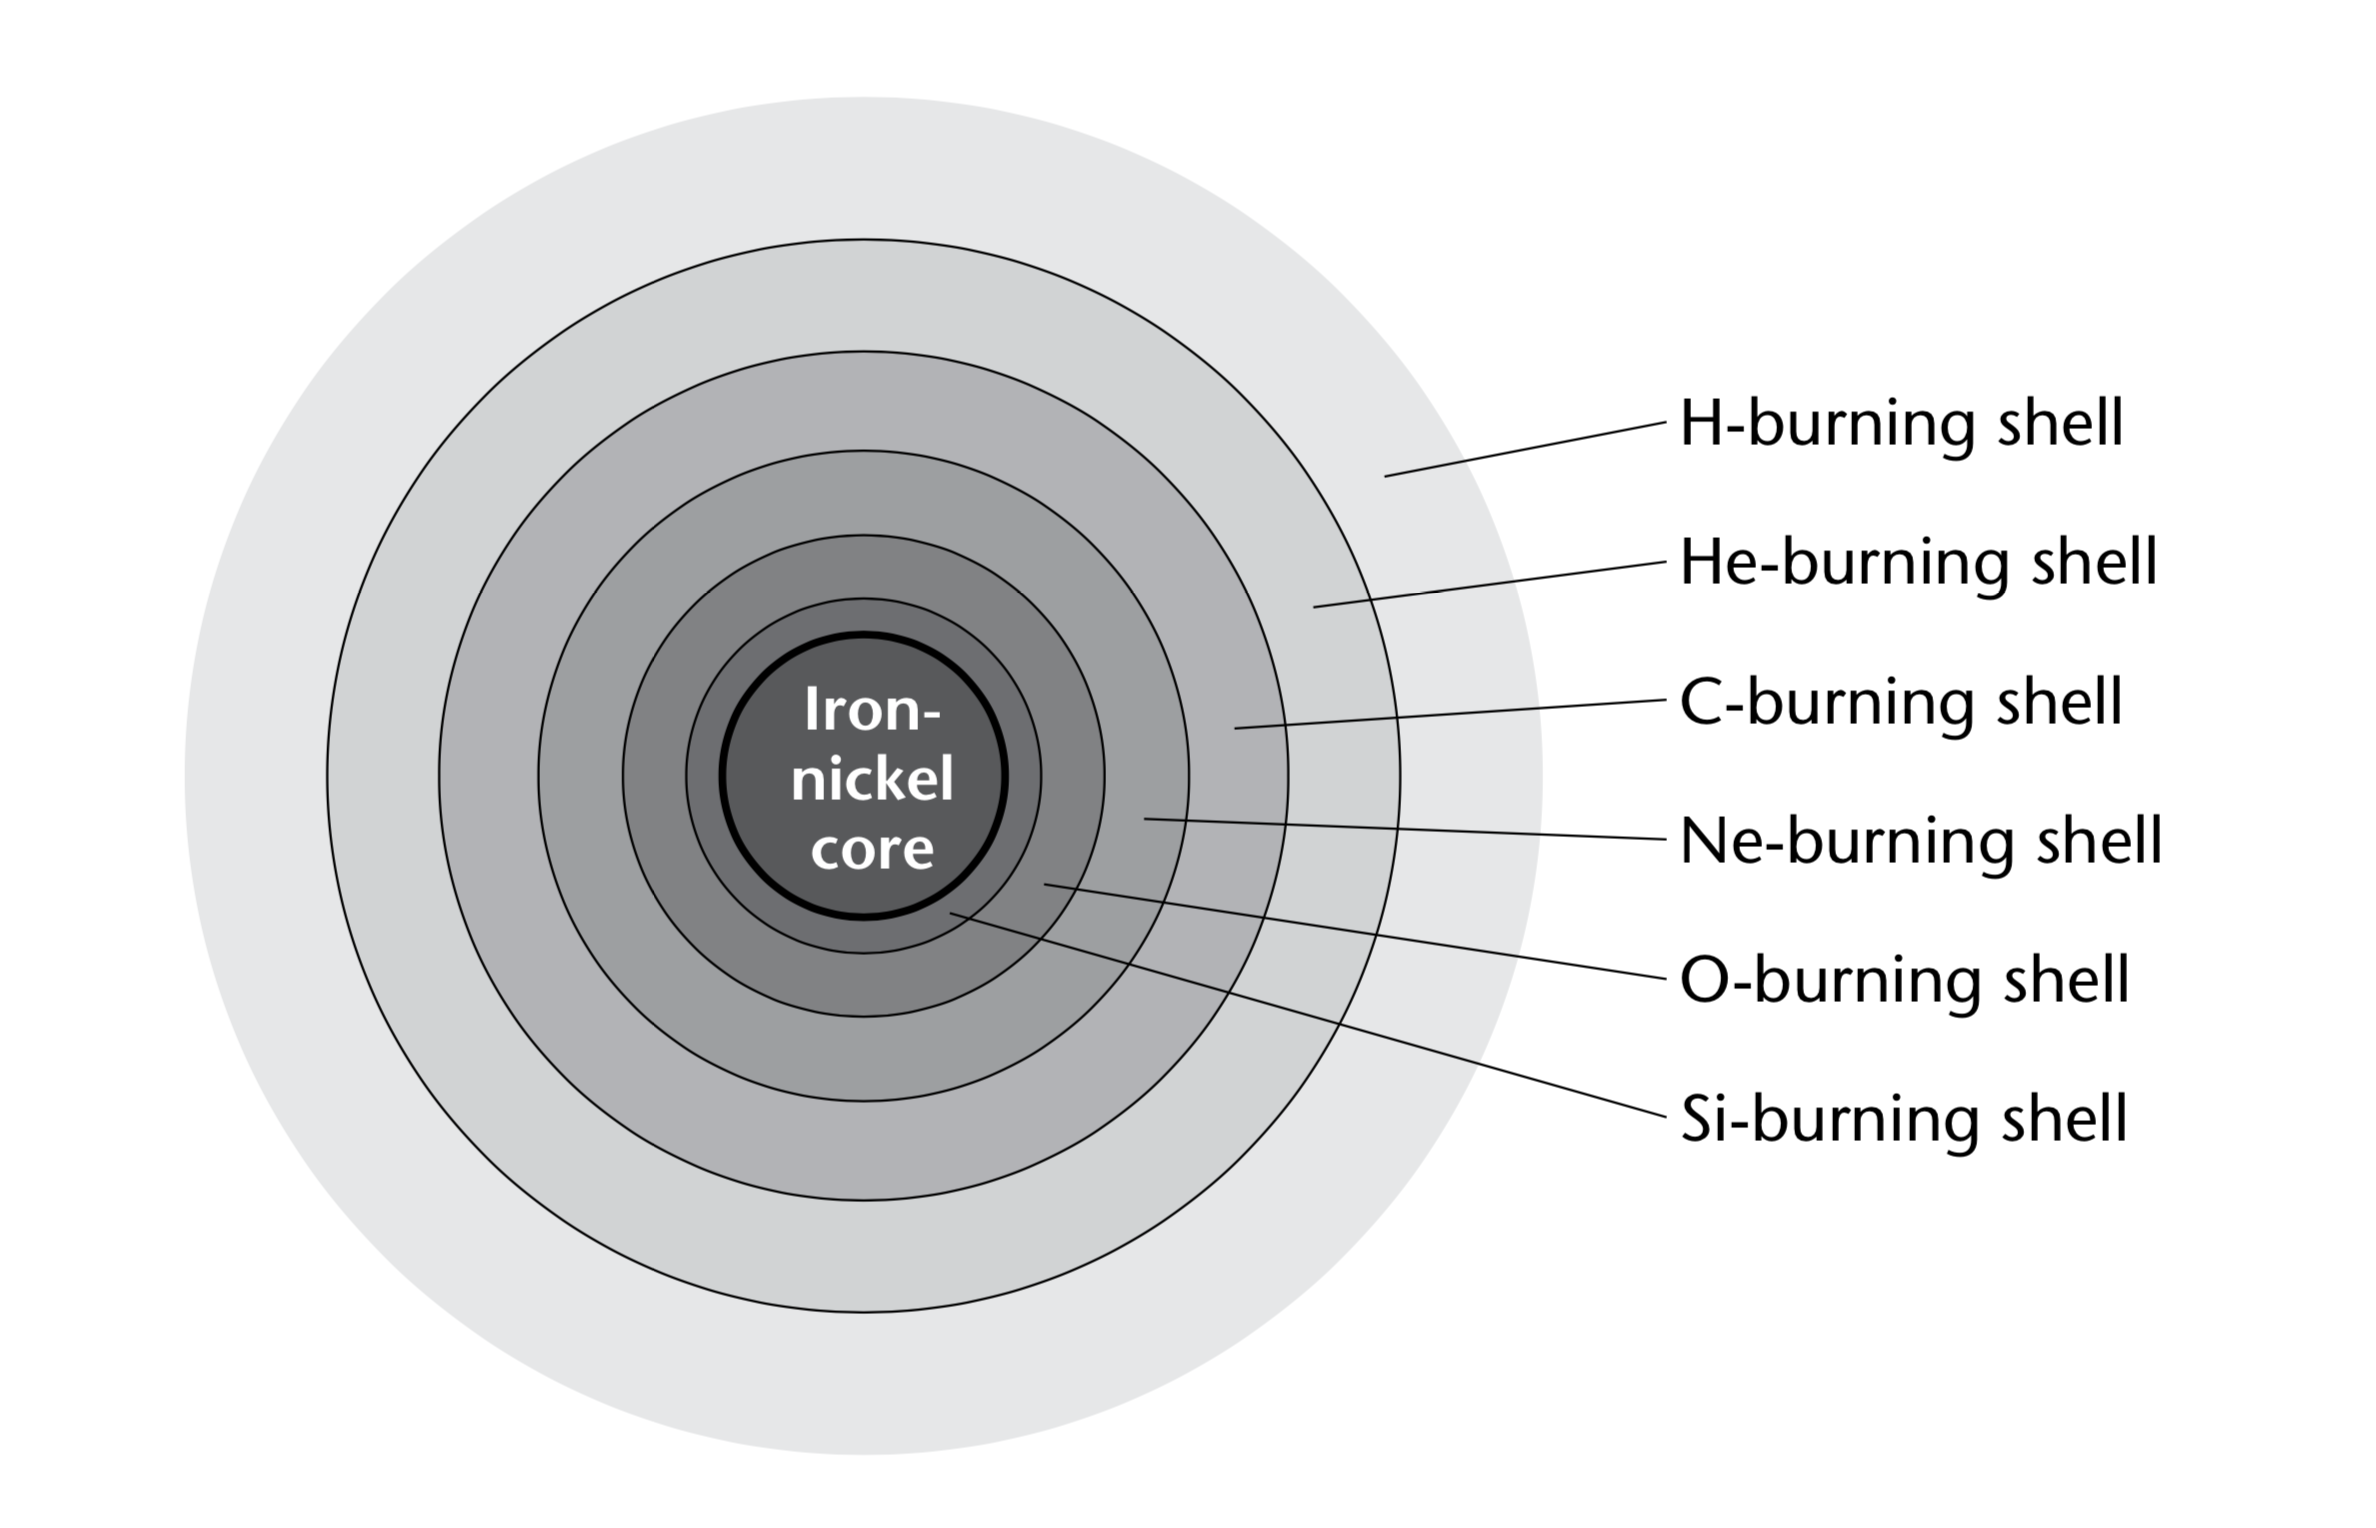
\includegraphics[width=\textwidth, angle=0]{Img/Onion-layer.png}
\caption{Schematic view of a massive star with over 8 M$_{\odot}$. At the end of its cosmic life, such star will have an iron-nickel core surrounded by layers of the recently produced elements. No more energy can be produced by iron fusion in its core. Credits: Peter Palm} 
\label{onion}
\end{figure}
 
\newpage

\section{Stellar Populations}
There are lots and lots of stars in our Milky Way, likely between 200 and 400 $\times 10^{9}$ stars \citep{2006S&T...111e..98R}. Section \ref{formation} assumes that our universe has an age of 13.8 $\times 10^{9}$ years (165.6 $\times 10^{9}$ months), making a roughly average of one birth per month. Elements are continuously synthesized in all this enormous number of stars, invariably driving chemical evolution onward. Sections \ref{formation} and \ref{evolution} discuss how stars form and evolve. However, the entire population of stars is like a bustling astronomical menagerie that includes quite a several unusual species besides any ingrained animals. In spite of the fact that it does not all the times appear as before-mentioned; at the moment you are looking at the sky or pictures of stars, there is enormous diversity with each other. Simply as in any handful of people or animals; stars can be classified as younger and elder (in term of age) or larger and smaller (in term of mass). In contrast, a star can change its size. All stars, near the end of their lives, expand toward an evolutionary phase knows as red giants. The red giant star "Betelgeuse \footnote{Betelgeuse is the tenth brightest star in the night sky before "Hadar" and after "Achernar", and the second-brightest in the constellation of Orion after "Alnilam". It is a reddish, semi-regular variable star, with apparent magnitude alters between +0.0 and +1.3.}", has a radius of 1,200 times our Sun's radius; because it is at its stellar deathbed \citep{2018A&A...609A..67K}. 

The stellar size of a star doesn't inevitably indicate anything about its stellar mass, in any case. However, stellar mass is an essential quantity in astrophysics. As an illustrative example, our Sun has a stellar mass of $2 \times 10^{30}$ kg \citep[roughly $3 \times 10^{5}$ the mass of Earth,][]{2017EGUGA..1911131E, 2019arXiv190612272C}, which serves as an astronomical unit to measure stellar masses (the so-called solar mass). Moreover, stellar masses have a broad range, the smallest stellar mass is about 0.1 solar mass; the minimum mass allows stars to ignite nuclear fusions at their cores. Usually, the term "low-mass star" refers to stars with stellar masses less than 2 M$_{\odot}$. Stars with stellar masses of 2-8 M$_{\odot}$ are "intermediate-mass stars". Stars with stellar masses of 8 or more M$_{\odot}$  are "massive stars". Low-mass stars are much more, number-wise, than massive ones. Statistically, for each massive star (M $<$ M$_{\odot}$), there are $10^{3}$ intermediate-mass and $10^{4}$ low-mass stars. The vast majority of the stars have stellar masses significantly less than 1 M$_{\odot}$; such as 0.3 M$_{\odot}$ or even lower \citep{2019MNRAS.487.2937O}.



The chemical composition of stellar objects is an often used distinguishing feature (the so-called  star metallicity; [Fe/H] \footnote{[A/B] = log(NA/NB)$\star$ - log(NA/NB)$\odot$, where N is the number density of atoms of a given element in the star ($\star$) and the Sun ($\odot$), respectively.}). The vast majority of stars have chemical compositions similar to that observed in our (metal-rich) Sun. However, few rare stars have lower metallicities$-$the poorer the star is, the more unique the star is; because it originates from the very early era of the universe, more than $10 \times 10^{9}$ years ago. These stars are know as metal-poor stars.


\subsection{The first stars}

As reported by many cosmological simulations, the very first stars were created in small mini-halos some several hundred million years later the Big Bang. The primordial gas, left after the Big Bang, lacked sufficient cooling agents (e.g., carbon, oxygen, and silicon); therefore, significant fragmentation was mainly overcome so that the first stellar objects were extremely massive  (of the order to ∼ 100 M$_{\odot}$). However, this is a different case compared with low-mass stars, ruling today’s mass function (IMF). These stellar objects are introduced as Population III or Pop III stars, as they have been formed from primordial (metal-free) gas \citep{1980A&A....83L..10P,1987Natur.326..829C,1988IAUS..126..701H,1990RMxAA..21..322D,2019MNRAS.487.3363W}. These stellar objects shortly exploded as supernovae (SNe) to either collapse into black holes \citep[progenitor masses of 25 $<$ M$_{\odot}$ $<$ 140 and M$_{\odot}$ $>$ 260) or to die as energetic pair-instability SNe (PISN; 140 $<$ M$_{\odot}$ $<$ 260;][]{2002ApJ...567..532H}). During their explosions, these stellar objects provided huge amounts of ionizing emissions (the PISNe also contributes some of the first metals) that altered the surrounding environment; hence the second generation (Population II or Pop II) stars might be less massive (M$\star$ $\sim$ 10 M$_{\odot}$) and long-lived object. 



Partially, the ionized stellar gas, which its chemical composition has been altered by the death of the first stars, will support the formation of H2 and the HD molecule. This, in turn, will facilitate additional effective cooling agents than what is available in zero-metal gas. In addition, the metals or the dust grains, which has been left behind from PISNe would have the same cooling effects as well. In spite of the fact that not all more massive SNe end in black hole creation. In spite of the fact that not all more massive SNe end in black hole creation, some massive (25 M$_{\odot}$) stars experience solely a partial fall- back; some of the lately synthesized metals get expelled into the surrounding stellar gas \citep[e.g.,][]{2003Natur.422..871U}. At that point, enough metals will present to guarantee enough gas fragmentation to support the low-mass ($<$1 M$_{\odot}$) star formation. These stars, which has been, formed from non-zero (any metal-enriched) stellar gas are known as Population II (Pop II) stars (see Figure \ref{star_cycle}). Besides, higher metal-rich stars (e.g., our Sun), which have been formed in more metal-rich environments are called Population I (Pop I). Stellar archaeology claims that the PopII stars preserve in their atmosphere the composition of the individual SN yields of the previous Pop III (the so called Pop III chemical fingerprint). Therefore, metal-poor stars can contribute to reveal the first nucleosynthesis enrichment in the universe \citep{2005ARA&A..43..531B, 2007ApJ...655..492A, 2016A&A...588A..37H, 2016ApJ...829L..24P, 2017MNRAS.471..404K,2017MNRAS.472..350R, 2018MNRAS.475.4781C,2018A&A...614A..68C,2019arXiv190409608M,2019ApJ...875...89M,2019arXiv190608439M}.



 

\begin{figure}[!ht]
\centering
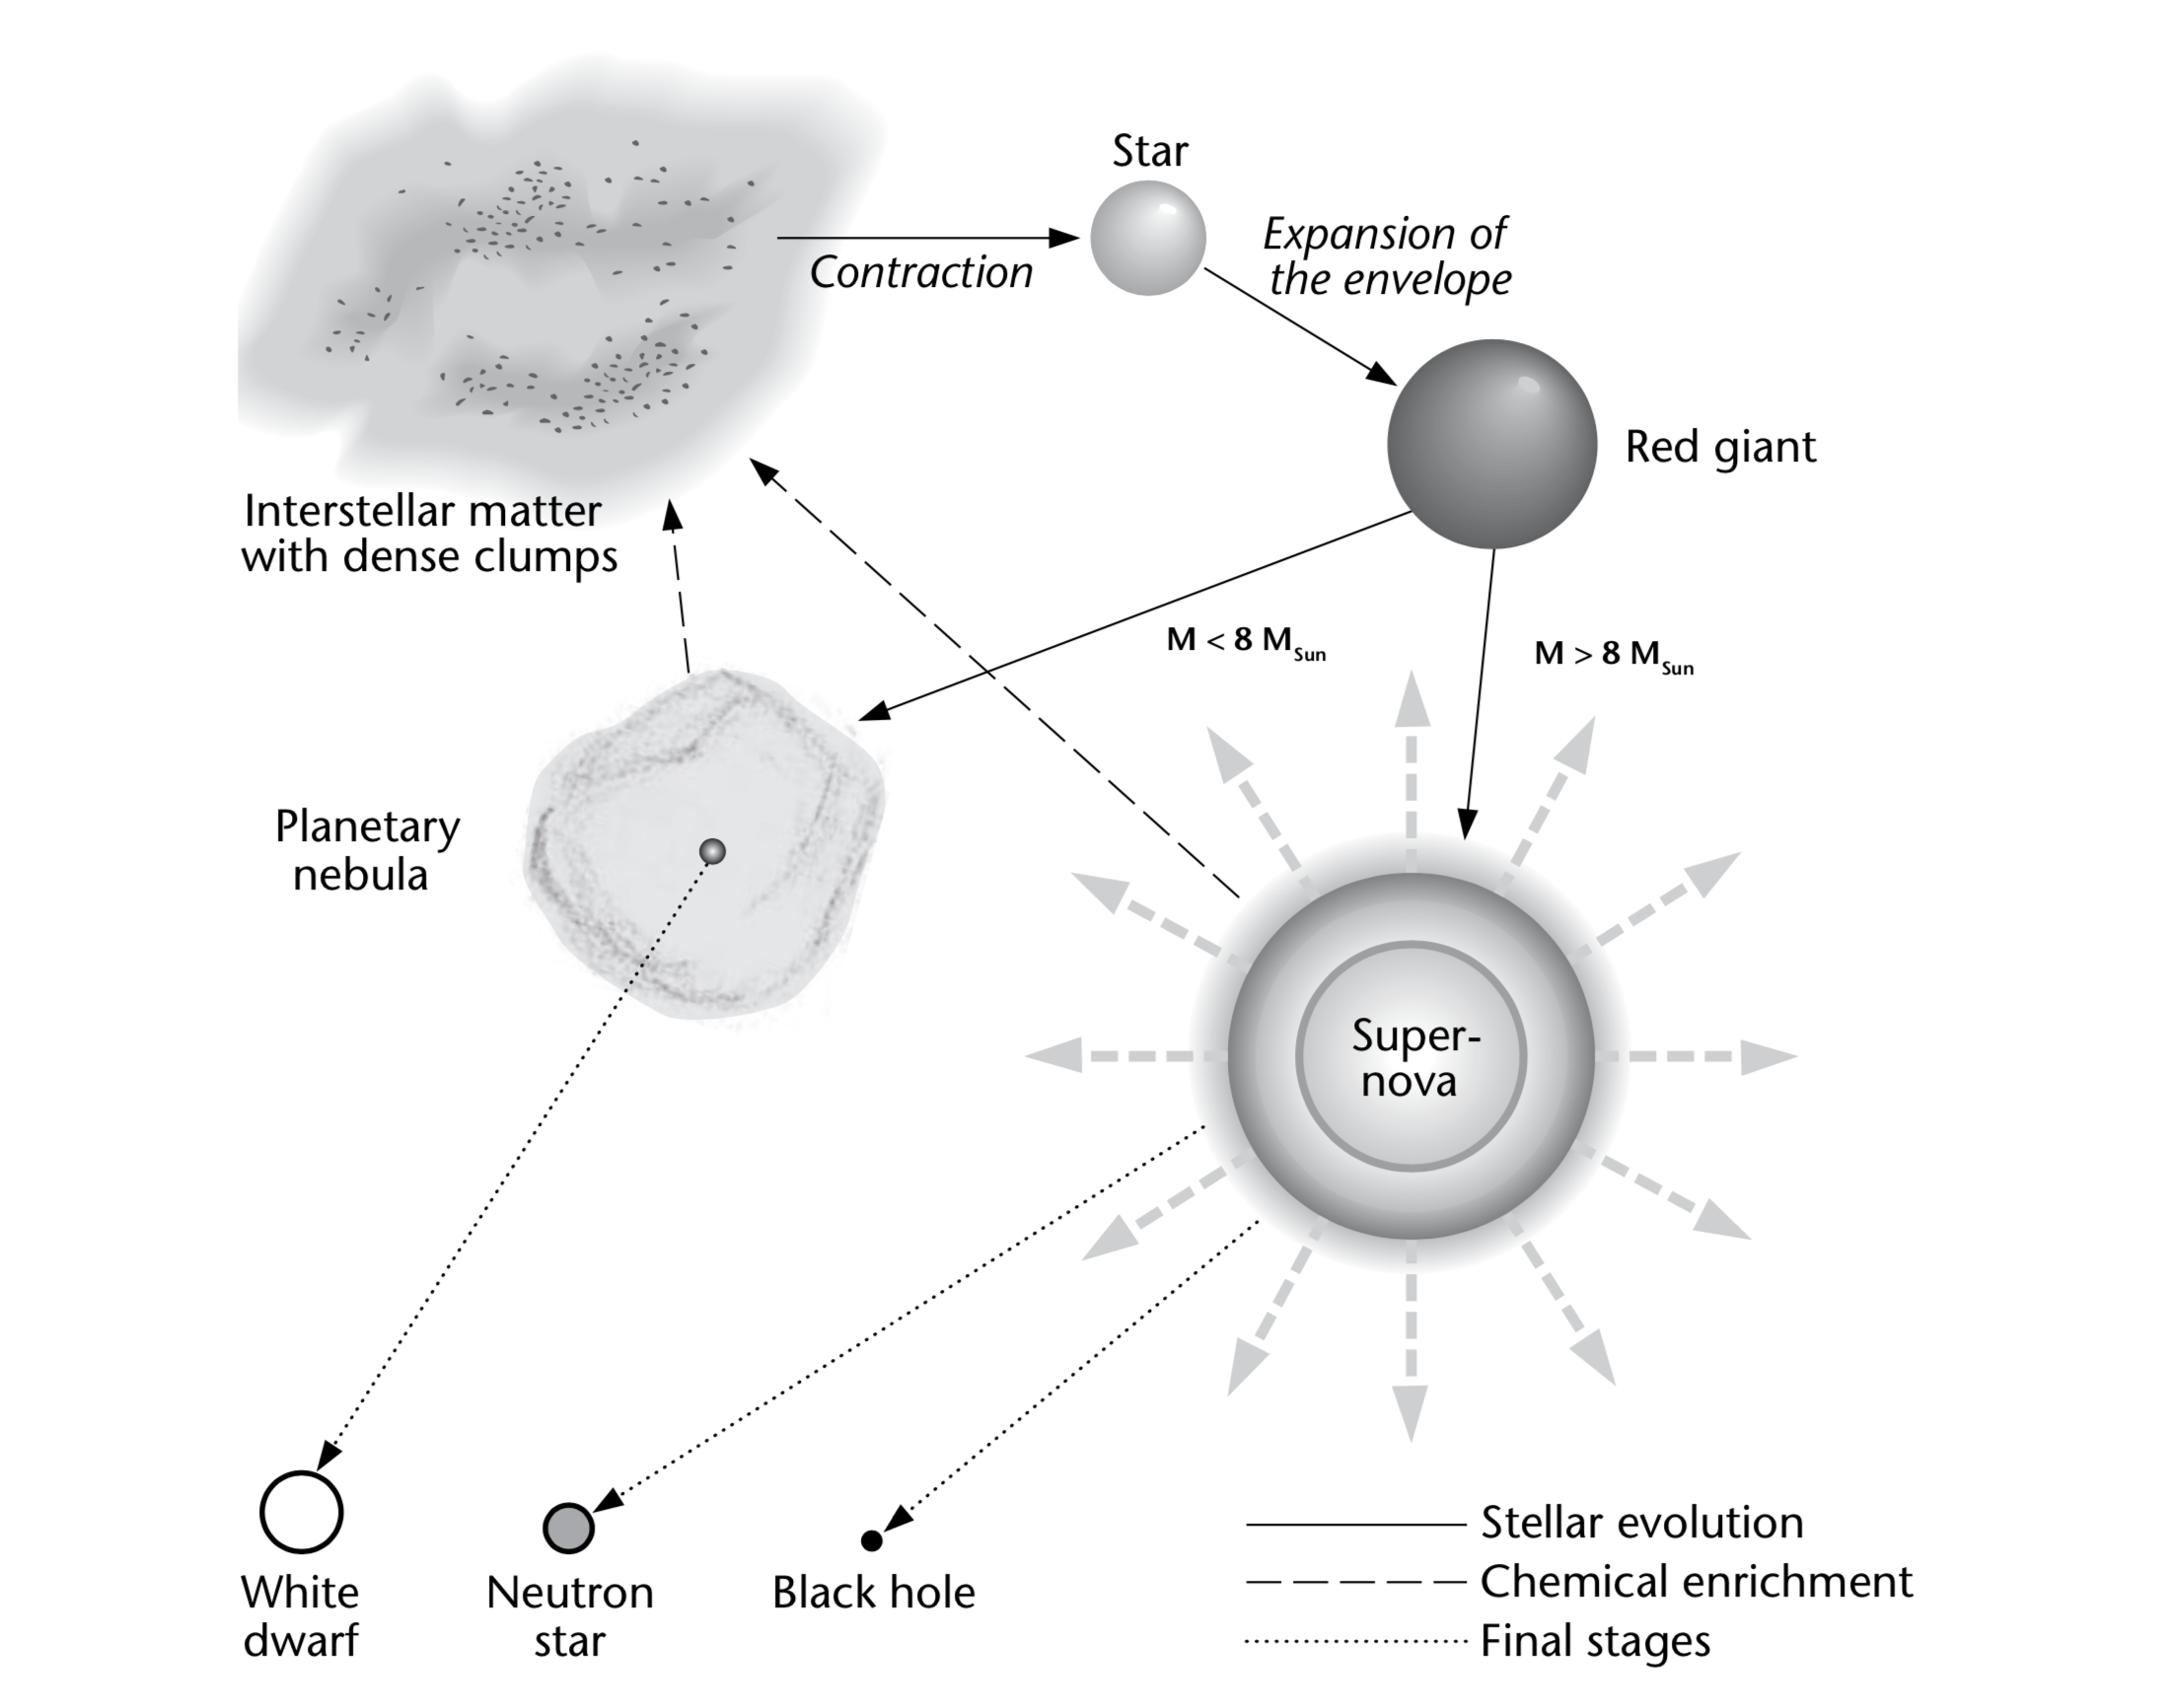
\includegraphics[width=\textwidth, angle=0]{Img/star_cycle.png}
\caption{Schematic view of the cosmic cycle of matter, stars will be formed from interstellar gas. The interstellar medium will be enriched by the elements synthesized in these stars, by either stellar winds or supernova explosions. Therefore, each successive generation of stars will be more metal-rich Credits: Peter Palm} 
\label{star_cycle}
\end{figure}


\subsection{Metal-poor stars}

We have mentioned that the first stars (pop III) have been formed from a pristine (zero-metal) gas cloud, shortly after the Big Bang. These stars were thought to be very massive; the absence of sufficient cooling agents \citep[e.g.,][]{2002ApJ...564...23B}. However, these stars exploded to enrich its surroundings and allow gas fragmentation to support the low-mass ($<$1 M$_{\odot}$) formation. The nowadays observed metal-poor stars belong to this stellar era. In their atmospheric surface, these stars store information about the chemical composition of their stellar gas cloud. They are providing archaeological data of the most primitive times of our universe. The chemical abundance patterns observed in their atmosphere present unique full information about the formation and evolution of our universe. These pieces of knowledge are valuable for the understanding of the galactic chemical evolution and formation. Metal-poor stars are our neighbors corresponding to the high-redshift universe \citep[e.g.,][]{2019arXiv190401615S}.



The justification for investigating metal-poor stars is that they are long-lived, low-mass stellar objects, the vast majority of the investigated metal-poor stars, in literature,  are main-sequence (MS) and giant stars that have not altered their atmospheric chemical composition and thus preserved the chemical signatures of their birth stellar gas cloud. Assuming that the entire universe was mostly lacking metals at its earliest eras, it is commonly believed (and carried out by investigation) that low metallicity star means and old age star; their masses are of order  0.6-0.8 M$_{\odot}$ (massive stars consume their fuels faster, therefore die more quickly). By analyzing the current chemical composition of their atmospheric surface, one can travel back in time to the early universe period and learn about its nature.  However, metal-poor stars can experience some internal mixing processes or accretion of interstellar material, which would alter the original atmospheric surface abundance. Such an assumption is vital in the metal-poor stars analyses. This field of study, in astronomy and astrophysics, is usually referred to as “near-field cosmology” or “stellar archaeology” \citep{2002Natur.419..904C, 2003Natur.422..871U, 2005Natur.434..871F, 2007ApJ...660..516T, 2010ApJ...724..341H, 2011Natur.477...67C, 2013ApJ...773...33I, 2013ARA&A..51..457N,
2014ApJ...790...34P,2014Natur.506..463K, 2014ApJ...785...98T, 2016A&A...586A.160H,  2018MNRAS.481.3838S, 2019arXiv190403211E}. The best candidates for such studies are the very metal-poor ([Fe/H] $< -2.0$, hereafter VMP), extremely metal-poor ([Fe/H] $< -3.0$, hereafter EMP), and  ultra metal-poor ([Fe/H] $< -4.0$, hereafter UMP) stars. These second-generation objects (Pop II) have formed from low-metallicity gas clouds at redshift $\gtrsim 6$


The ultimate rationale for studying metal-poor is to gain insights into the early universe. However, still there are many other justifications, here we try to mention the most important of these reasons for analyzing metal-poor stars. 


\begin{enumerate}
  \item The most metal-deficient stars (ultra metal-poor), with no enhancement in the heavy elements (Z > 3) abundances, are believed to be the most primitive stars observed until now.
  \item The lithium (Z = 3) abundances observed in main-sequence-turnoff extreme metal-poor ([Fe/H] $<-$3) have the great potential to place direct constraints on the physical and chemical conditions of the Big Bang.
  \item The redshifts epochs $> 6$ are believed to be the era where the most metal-deficient stellar objects have been formed, and the best candidate to examine the physical and chemical conditions at the time the very first heavy element was built. 
  \item Metal-poor stars constrain our perception of the nature of the very first stars (Pop III), the initial mass function (IMF), the explosion of supernovae, and how the Pop III ejecta was incorporated into succeeding early stars.
  \item The direct comparison of the predicted yields of stellar evolution models and/or the galactic chemical enrichment scenarios significantly constrain the science of the creation and development of the very first stars/galaxies.
  \item Some of the metal-poor stars ([Fe/H] $\sim 3.0$) show strong enhancements in the neutron-capture elements, that the detection of Th (Z= 90) and U (Z= 92)  is likely possible and thus the estimation of their age and the universe. 
  \item Metal-Poor stars with [Fe/H] $-0.5$ (Hyper metal-poor) acquaint our perception of the Milky Way growth; the connections between chemical abundance, kinematics and dynamics, and the age distributions, the defining properties of stellar groups,  allow votes among the different models of how the Milky Way system formed and has grown.
\end{enumerate}


\subsection{The diversity of the observed chemical abundances of metal-poor stars}

For a long, long time, we believed that all field stars would likely show chemical composition similar to our Sun. This assumption came to its end in the mid of the nineteenth century (1940), at the moment that some metal lines detected in stars seemed to be surprisingly weak corresponded with our Sun. The first explanation was that these stars would have peculiar atmospheres or they are hydrogen-deficient stars. However, \citet{1951ApJ...114...52C} presumed that these unique stars would be the foresight of abnormally low amounts of calcium and iron, in their work, they found $\sim$ 1/20th the solar values. Following studies on before-mentioned stars through the subsequent few decades proved that some stars do certainly have different metallicities that reveal various phases of the chemical evolution experienced by our Milky Way. \citet{1951ApJ...114...52C} observed many stars, including HD140282, which has been a point of many studies in the previous half-century.  For example, \citet{2001ApJ...561.1034N} studied HD140282 and reported that this subgiant star has peculiar chemical composition with [Fe/H]=2.5. For the convenience of the reader, and the view of this thesis, the term "metal-poor" will be considered to indicate any low metalicity ([Fe/H] $< -1.0$) object, in our Milky Way; to include all of the metal-poor stars' categories by one term.


Metal-poor stars are significant for constraining and explaining the creation history of our Milky Way, in addition to the physics of the high redshift universe (e.g., initial mass function).  The general strategy is to collect such knowledge through the study of the complete elemental abundances patterns of metal-poor stars; many of these stellar objects built from the primordial (zero-metal) gas clouds throughout the very early chemodynamical growth of our galaxy \citep[e.g.,][]{2005ARA&A..43..531B}. Many Chemical abundance analyses of these metal-poor stars present valuable constraints on the appropriate nucleosynthesis rules and the chemodynamical growth of our early galaxy \citep{1990A&AS...86...85Z,1991A&A...244..425Z,1995AJ....109.2757M,1998AJ....115.1640M,2004A&A...416.1117C,2005A&A...435..373B,2008ApJ...672..320C}. Recently, notable attempts have been performed to fully describe the metallicity distribution function (MDF) of the halo system, particularly at the very metal-poor end (e.g., the HK survey and the Hamburg/ESO).  These survays yielded an exciting development in known metal-poor stars. High-resolution spectroscopic investigations of these stars distinguished in the Hamburg/ESO survey have proved the presence of ultra and hyper metal-poor stars in the halo system \citep{2002Natur.419..904C,2005Natur.434..871F,2007ApJ...670..774N}. All these discovered stars are carbon-rich stars; no entirely metal-free (compose of only hydrogen and helium) stars have been observed thus far. Their results could be employed to place crucial constraints on the IMF.
For illustration, semi-analytic models of Galaxy formation show that the absence of zero-metal stars restrains the crucial metallicity should be  Z$_{cr} > 0$  for low-mass stars formation \citep{2002ApJ...571...30S,2007MNRAS.381..647S}.



The full detailed elemental abundance patterns analysis of metal-poor stars can provide more valuable information on the chemical history of the halo system; different processes synthesize various elements, in different masses and timescales. As an illustrative example, $\alpha$-elements (nuclei with atomic number integer multiples of four; O, Mg, Si, Ca, and sometimes Ti) built during explosions of massive stars (M$_{\star} < 8$ M$_{\odot}$), just several million years, after their formation. In contrast, iron-peak elements (local peak in the region of iron; Cr, Mn, Fe, Co, and Ni) are synthesized either by Type Ia or Type II supernovae. Moreover, Type Ia supernova is the outcome of the thermonuclear explosion caused by mass transfer onto the surface of a white dwarf star by its companion star, in a binary system, or a consequence of a white dwarf$-$white dwarf (double-degenerate) collisions, and thus occur on a more protracted timescale, of the order of 0.1 to few Gyr \citep{2001ApJ...558..351M}. A more extreme example is the Heavy elements (beyond the iron-peak) production. These elements are built by neutron captures; through the slow (s) furthermore rapid (r) processes. The vast majority of these metal-poor stars show high $\alpha$-enhancement \citep[typically $\alpha$-to-iron ratio $\sim$ $+0.4$,][]{1989ARA&A..27..279W, 1994A&A...285..440N, 2000A&A...356..238C}.



Another different possible chemical patterns, observed in metal-poor stars, are the carbon-rich or carbon-enhanced metal-poor \citep[CEMP; carbon-to-iron ratio $> 1.0$ dex][]{2005ARA&A..43..531B} stars. A number of previous observational studies have indicated that carbon is
omnipresent in the early universe \citep{2005ARA&A..43..531B,
2007ApJ...655..492A, 2016A&A...588A..37H, 2016ApJ...829L..24P,
2018MNRAS.475.4781C, 2018A&A...614A..68C}. Hence, the discovery and analysis of
carbon-enhanced metal-poor stars ([C/Fe] $\geqslant 0.7$\footnote{Using
\citet{2007ApJ...655..492A}, as the criterion for carbon enhancement.}
hereafter CEMP), suggest that this substantial enhancement could be closely
linked to their formation.  In addition to carbon enhancement, different
abundance ratios of neutron-capture elements are often used to distinguish the
unique nature of CEMP stars:  CEMP-s ([C/Fe] $\geqslant +0.7$, [Ba/Fe] $>
+1.0$, and [Ba/Eu] $> +0.5$),  CEMP-r/s ([C/Fe] $\geqslant +0.7$ and $0.0 <$
[Ba/Eu] $< +0.5$),  CEMP-r ([C/Fe] $\geqslant +0.7$ and [Eu/Fe] $> +1.0$), and
CEMP-no ([C/Fe] $\geqslant +0.7$ and [Ba/Fe] $< 0.0$).

The CEMP-s and CEMP-no subclasses represent the predominant populations of the
CEMP stars \citep{2005ARA&A..43..531B, 2007ApJ...655..492A,
2016A&A...588A..37H,  2016ApJ...833...20Y}. The chemical patterns associated
with CEMP-s stars (high enhancement in carbon and s-process elements) can arise
from an intrinsic (self-enrichment) or an extrinsic (mass transfer from now
white dwarf companion) process. Nevertheless, the overabundance of s-process
elements (e.g., [Ba/Fe] $> +1.0$) support the matter accretion from an
asymptotic giant branch (AGB) companion. These s-process elements
(e.g., Sr, Ba, and Ce) are believed to be synthesized in low- to
intermediate-mass stars (1 to 3 M$_{\odot}$), with low neutron densities ($n_{n}
\approx 10^{6} $ cm $^{-3} - 10^{10}$ cm $^{-3}$) and $^{13}$C($\alpha,
n$)$^{16}$O as the main source of neutrons, which are eventually
transferred and mixed into the atmosphere of the long-lived companion
\citep[observed as a CEMP-s star,][]{2005ApJ...625..825L,
2014MNRAS.441.1217S}. 
 
CEMP-r/s and CEMP-r are much less frequent when compared with other subclasses.
The origin of their enhancement (in r-process elements) is still widely
debated. In contrast to the s-process elements, a high neutron density ($n_{n}
> 10^{22}$ cm $^{-3}$) is the key to synthesize these
unstable neutron-rich isotopes (e.g., Eu, Os, and Ir). In the past, there have
been many astrophysical sites proposed for r-process production. Still a few
can provide such high neutron density environment \citep[see][and references
therein]{2017ARNPS..67..253T}. Presently, the possible sites are confined to
magnetorotationally jet-driven supernovae (SN), core-collapse SN, neutron
stars mergers, and neutron star-black hole mergers
\citep[e.g.,][]{2018ARNPS..68..237F}.
 
The CEMP-no stars, which are believed to be the direct descendants of objects
formed shortly after the big bang (Pop III), \citep{2013ApJ...773...33I,
2014ApJ...790...34P,2016A&A...586A.160H}, dominate the lowest-metallicity regime
(e.g., \citealt{2002Natur.419..904C, 2005Natur.434..871F, 2011Natur.477...67C,
2014Natur.506..463K, 2018MNRAS.481.3838S}) and reside in the main-sequence,
subgiants, or red giant phase.  Their evolutionary stages and chemical patterns
(excess in carbon with low abundances or absence of neutron-capture elements)
suggest that a binary companion or self-enrichment are unlikely the sources of
their chemical patterns. Therefore, a distinct enrichment channel may have
taken place (e.g., \citealt{2014MNRAS.441.1217S, 2016A&A...588A...3H}).
A spinstar is one possible candidate; these rapidly rotating
massive ultra metal-poor ([Fe/H] $< -6.0$) stars can produce large
amounts of carbon \citep{2006A&A...447..623M, 2007A&A...461..571H,
2012A&A...538L...2F, 2015A&A...576A..56M}.  Another proposed scenario for the
carbon enhancement is pollution from faint supernovae associated with Pop III
stars, with mixing-and-fallback \citep{2003Natur.422..871U,
2007ApJ...660..516T, 2010ApJ...724..341H, 2013ARA&A..51..457N,
2014ApJ...785...98T,2019arXiv190403211E}. This faint SN ejects less iron and
thus increases the [C/Fe] ratio, as they do not have enough energy to eject all
its material into its surroundings. Therefore, only the outer layers with the
lightest elements are ejected while the inner part falls back onto the neutron
star or black hole.  At present, none of the above scenarios can explain the
full chemical patterns that have been observed in CEMP-no stars.In
general, the unique chemical patterns observed in the sub-classes of CEMP stars
result from the differences in the astrophysical sites responsible for the
nucleosynthesis products they now mixed in their atmospheres.




\section{The structure of the Milky Way system}


We live/exist inside the Milky Way (our Galaxy). Therefore, cosmologists have long attempted to place constraints models on its formation and evolution. However, the glimpse into the cosmos is regrettably somewhat restricted, and thus, creativity is required to figure out what our Galaxy might indeed look like and what it is composed of. Because of its huge size, we would never be capable of viewing its whole shape neither. Nevertheless,  many observations of other galaxies \citep[e.g.,][Andromeda galaxy,]{2005ApJ...635L..37R} might provide some clues to this vital puzzle. Many ancient civilizations investigated the night sky by the most primitive optical tools (the human eye), to have a similar view, we have to move to the countryside (no light pollution) at a dark night(no bright moonshine). The scene will be somewhat like that the vast majority of our galaxy's stars assembled in a broad, scattered stripe crossed the sky \citep{2015hae..book.1549J}. 

Going back in time, the famous womanizer and the chief of all Greeks' gods Zeus had procreated a son, Heracles. Zeus' wife, the goddess Hera, was loaded with anger and jealousy. Heracles was not immortal such as the rest of the Greeks' gods; Heracles' mother was a mortal woman. Therefore, the king Zeus resorted to some cunning to cure this flaw; breastfeeding him from Hera was supposed to help, the baby boy, Heracles to earn his immortality. Thus the king Zeus, secretly, used to place Heracles with Hera while she is sleeping. However, the newborn nursed so vigorously and woke Hera up. With anger as hell, Hera threw Heracles away from her breast, that Hera's milk was sprayed all the way up to the heavens, where it seems as the Milky Way \citep{2019AAS...23314620T}. A beautiful small myth to include in this thesis, yet what is the Milky Way in reality?


Few years after the invention of the telescope (around 1600 AC), Galileo Galilei (Italian scientist and inventor) investigated the Milky Way with the recently invented telescope, thus holding all the credits of this pioneering idea \citep{2010JHA....41..120B}. In his examination, he found that the glittering band across the sky composed of countless numbers of faint stars. Three centuries later, William Herschel (English astronomer) examined the night sky and published the first map of  the Milky Way. This map shows how our galaxy might look like from a far distance. Nowadays, we acknowledge that the vast majority of the Milky Way's stars gathered inside a flat plate that gives the original appearance of the Milky Way \citep{2018JAHH...21..251C}. Apart from this, what makes these stars order themselves in this unique way?

Many astronomers around 1900 did more and more investigations on the Milky Way's structure, using some stellar statistical techniques, which proved its difficulty \citep{1910KNAB...13..239P,1912JRASC...6..225E,1922HarCi.242....6B,1936PA.....44..466P,1939HarCi.424....1B,1943PhDT.........2M,1950Natur.165..487B,2018RAA....18..146X,2019MNRAS.487.1400C}. However, the situation changed at the time Henrietta Leavitt (American astronomer) made her significant discovery \citep[period-luminosity relation,][]{1908AnHar..60...87L,1912HarCi.173....1L} and finally gave the right means for the progress. A few years later, Harlow Shapley (American astronomer) employed her period-luminosity relation to making the Cepheids' distance measurement, thus establishing the technique of measuring stellar structures' distances inside and outside the Milky Way, as long as Cepheids exist nearby \citep{1927HarCi.314....1S}. Afterward, Jan Oort (Dutch astronomer) succeeded to explain and describe our galaxy's motions with geometry and several targeted observations \citep{1927BAN.....4...79O}. In his study, he found that the Milky Way's stars rotate around its center due to a gravitation force, caused by a heavily compressed mass at its center. Therefore, these stars organized in a disk and act similar to a fluid that revolves slower at the edge than its center. It has primarily been recognized that our galaxy has a complete spiral structure; all the disk's stellar objects (stars, gas, and dust) arranged in several spiral arms. The following years presented innumerable observational evidence that permanently established our galaxy's disk-like shape \citep{2018ApJ...859L...8H}. Moreover, Radio-astronomers detected the preliminary component of the spiral arms (hydrogen gas). As a result, the Milky Way is, now, widely acknowledged as an example of a spiral galaxy such as many other galaxies \citep[e.g.,] [Andromeda and NGC 6744]{2017PhDT........53Y}.

To create an imaginary idea of our home galaxy, we can imagine it as a very dense griddlecake, with generous coats of jelly jam and cream cover the top and bottom, fulfilled by a centrally located scoop of ice-cream, before serving to Rufina (my beloved girlfriend) add a cherry on the tip of the ice-cream scoop. The jelly jam and cream express various stellar populations spread over our Galaxy's disk that add to the giddlecake's thickness. The ice-cream scoop represents our Galaxy's bulge; large, dense, and the most luminous part of our home galaxy. Many observations show that the spiral arms of the Milky Way, in the inner part, merge to form one bar-shaped structure. At the precise middle of the Milky Way's bulge, there is an overwhelming-massive black hole of $4 \times 10^{6}$ M$_{\odot}$; the cherry (see Figure \ref{milkyway}). This monster black hole swallows enormous quantities of stellar objects (e.g., stars and gas). 

\vspace{5mm}
\begin{figure}[!ht]
\centering
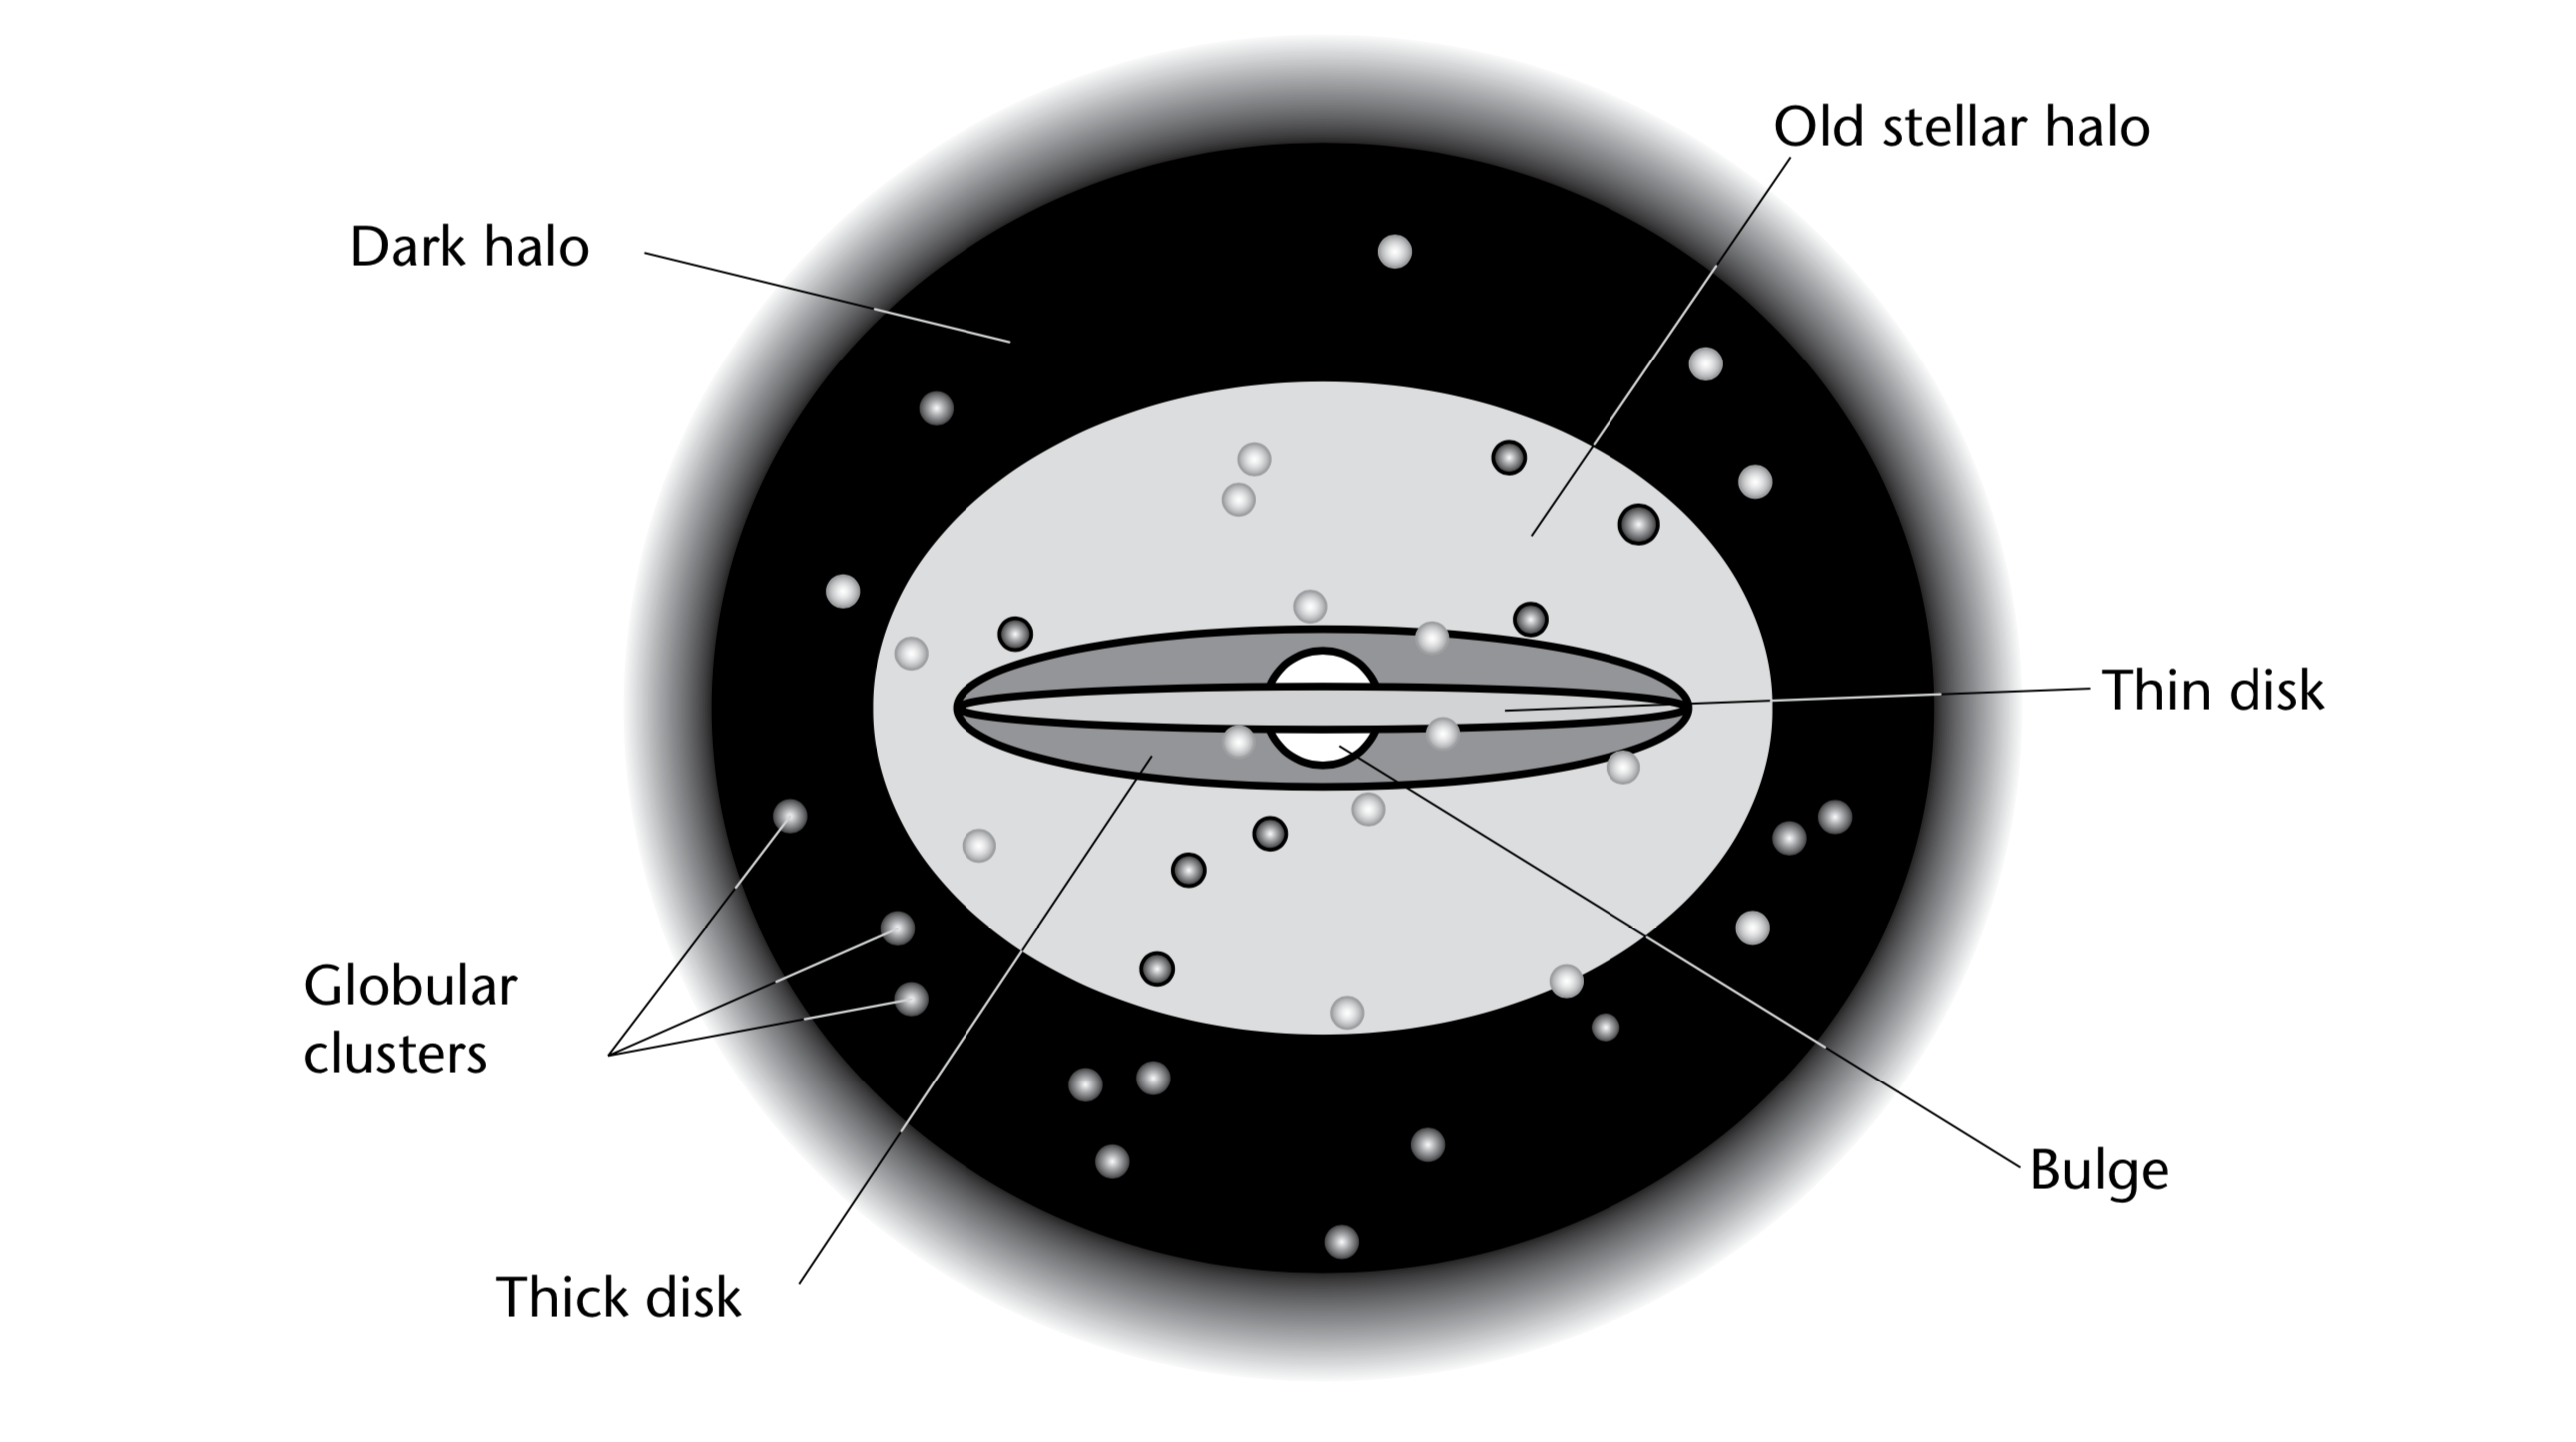
\includegraphics[width=\textwidth, angle=0]{Img/milkyway.png}
\caption{Schematic view of of the Milky Way with its different components indicated. Credits: Peter Palm} 
\label{milkyway}
\end{figure}


\vspace{5mm}


The Milky Way's disk (thick disk, thin disk, and spiral arms)  cover a wide area, with 100,000 light-years (ly) diameter, 1,000 ly thick, and 1,000 ly length \citep{2019A&A...625A.105H}. Our home (the Solar System) is located far away (With respect to the Milky Way's center) in the disk thus the overwhelming-massive black hole creates no threat to our existence. As long as the Earth is orbiting our Sun with a velocity of 30 km/s, the Sun (with the whole Solar System) inside the spiral arm, which it is located at (the Orion-Cygnus Arm)\footnote{Our exact position in the Milky Way is in the local spiral arm that is also referred to as the Orion-Cygnus Arm. The Sun and the Solar System lie at the inner edge of this arm. There are four larger and two smaller arms in total. The spiral arm laying in the direction of the center, seen from us, is the Sagittarius Arm, and the one behind us is called the Perseus Arm.}, is revolving around the Milky Way's center, with a velocity of 220 km/s and a somewhat an elliptic orbit. With its 4.6 billion years of age, the Sun has accordingly revolved approximately 20 times around the Milky Way's center that our existence (mammals; came to life somewhat 200 million years ago) does not yet represent to one Galactic revolution (Galactic year). 

\vspace{3mm}
Our sky view is somehow restricted; we live inside the Orion-Cygnus arm. Thus we would be able to observe part of the remaining spiral arms as well as stars and gas from our spiral arm. However, our galaxy approximately divides the sky into two identical regions; the Solar System located in the central plane of the galactic disk. Therefore, when we observe upward or downward, we would be able to see outside the Milky Way. However, we will not see anything except the Milky Way band around us at the moment we look along the galactic disk's plane. This Milky Way band is the result of the spiral structure of the galactic disk;  the view of Northern Hemisphere is directly towards the Perseus Arm, while the sight of Southern Hemisphere is directly towards the Sagittarius arm along the galactic center making it looks even more magnificent.


By having a more substantial look at our galaxy on the sky, we will immediately notice that it consist of small and large bright regions rather than being homogeneously lit up. Dark zones intermittent with the lighter ones, and the number of the observable stars can be inconstant. Interstellar dust and gas clouds cause these dark regions (Coalsack)\footnote{Coalsack is a stellar region where stars light, on its way to us, is entirely blocked by very dense interstellar dust and gas clouds.}. The galactic disk contains enormous amounts of the stellar dust; particularly at the stellar site(s) where star formation took place. Dust assists star formation; cooling agent, allowing the stellar gas cloud to clump and compress into a star. Furthermore, the only way to observe the galactic center is only by employing radio astronomy.

Young stars densely populate the disk of the Milky Way; $95\%$ of all Galactic stars. The galactic disk is made up by the so-called the thick disk, which surrounds a more substantial part, so-called thin disk (see Figure \ref{milkyway}; demonstrating the distinguished disks). The disk parts are enclosed in a huge sphere; the stellar halo. The galactic halo has a significantly less star's density than the galactic disk and mainly contains some old stars, star clusters, and dwarf galaxies. This stellar system is uniquely crucial for galactic archaeology; it hosts the oldest and most metal-poor stars. All halo objects rotate around the galactic center, with large reasonably circular orbits. The galactic halo spreads around the Milky Way over several hundred thousands light-years.


Metal poor stars reside primarily in the halo system of the Milky Way, a complex old component of the Galaxy that comprises at least two diffuse stellar populations, the inner- and the outer-halo, with different metallicities, kinematics and spatial density profiles \citep{2007Natur.450.1020C, 2010ApJ...712..692C, 2012AAS...21922206B}, several streams and overdensities \citep{2009ApJ...693.1118G}, and a recently discovered large structure in the inner region, product of a past merger event \citep{2018Natur.563...85H}. It has been recognized that 15\% $-$ 20\% of stars with [Fe/H] $< -$2.0 in the halo system are CEMP and the fraction increases with declining metallicity becoming $\sim$ 75\% at [Fe/H] $< -$4.0  \citep[see][and reference therein]{2014ApJ...788..180C}. There is also evidence for a significant contrast in the frequency of CEMP stars that are kinematically assigned to the inner- and outer-halo components (the inner halo is on-average non rotating, while the outer halo exhibits a significant retrograde signature). The outer halo exhibits a fraction of CEMP stars twice the inner halo in the metallicity interval $-$2.5 $<$[Fe/H] $-$2.0 \citep{2012ApJ...744..195C}. Such increase in frequency of CEMP stars can be explained as a population driven effect, due to the fact that the outer halo is the dominant component at large distance from the galactic plane and at metallicities, [Fe/H] $< -$2.0. The chemical differences between the two stellar halo populations were established also in terms of CEMP sub-classes by \citet{2014ApJ...788..180C}. It was shown that the relative numbers of CEMP-no stars compared to CEMP-s varies between the inner- and outer-halo and the frequency of the CEMP-no stars is higher in the outer halo, while the frequency of the CEMP-s stars is higher in the inner halo. The analyses of kinematics and dynamics of our sample stars will establish their inner/outer halo membership and on their origin. The chemical abundance analysis of metal-poor stars and searching of CEMP and NEMP stars provides important constrains on the chemistry evolution of the Galaxy, initial mass function (IMF; \citealt{2014ApJ...781...60H}) and the models of mass-transfer and evolution of components in binary systems.